\documentclass[a4paper, 12pt]{article}

\newcommand{\languages}{french, english}

\input{include/head.tex}

%%%%%%%%%%%%%%%%%%%

\newcommand{\imgheader}{resources/pdf/logo-uliege.pdf}
\newcommand{\institution}{Université de Liège}

\title{Étude statistique des taux de natalité et mortalité dans différents pays du monde}
\newcommand{\subtitle}{Élément de statistiques}

\newcommand{\group}{\textit{Groupe 19}}
\author{Bastien \textsc{Hoffmann} (20161283)\\Maxime \textsc{Meurisse} (20161278)\\}

\newcommand{\context}{3\ieme{} année de Bachelier ingénieur civil}
\date{Année académique 2018-2019}

%%%%%%%%%%%%%%%%%%%

\renewcommand{\thesubsection}{\thesection.\alph{subsection}}
\renewcommand{\thesubsubsection}{\thesubsection.\roman{subsubsection}}

\newcommand{\T}{\mathcal{T}}
\newcommand{\X}{\mathcal{X}}

%%%%%%%%%%%%%%%%%%%

\begin{document}
    % ---------- Page de garde ---------- %
	\newgeometry{margin = 2.5cm}
\makeatletter
\begin{titlepage}
	\begin{minipage}[t][0.425\textheight][t]{\textwidth}
		\begin{center}
			\includegraphics[height=0.15\textheight]{\imgheader}
			\vfill
			{\huge \textsc{\institution}}
			\vfill
		\end{center}
	\end{minipage}
	\vfill
	\begin{minipage}{\textwidth}
		\hspace{6pt}
		\begin{mdframed}[linewidth = 2pt, innertopmargin = 12pt, innerbottommargin = 12pt, leftline = false, rightline = false]
			\begin{center}
				{\LARGE \bfseries \@title}
			\end{center}
		\end{mdframed}
		\hspace{6pt}
	\end{minipage}
	\vfill
	\begin{minipage}[b][0.425\textheight][t]{\textwidth}
		\begin{center}
			{\LARGE \subtitle}
			\vfill
			{\large \group}
			\vskip 0.5cm
			{\large \@author\space}
			\vfill
			{\large \context \\[6pt] \@date}
		\end{center}
	\end{minipage}
\end{titlepage}
\makeatother
\restoregeometry
	
	
	% ---------- Analyse descriptive ---------- %
	\section{Analyse descriptive}
	
	% Question 1 - a)
	\subsection{Histogrammes des taux de natalité et de mortalité}
	\label{subsec:Q1a}
	On travaille sur une base de données de \num{100} pays contenant leur nombre de naissances et de décès (par \num{1000} habitants) en 2013. Les histogrammes, dont les taux en abscisse sont en \textperthousand\footnote{Tous les taux de ce rapport, et notamment ceux des figures, même si cela n'est pas partout précisé et sauf indication contraire, sont en \textperthousand.}, ont été générés par le script \hyperref[subsec:code-Q1]{\texttt{Q1a}}\footnote{Tous les scripts et fonctions mentionnés dans ce rapport se trouvent en annexe et ont été exécutés via le logiciel \href{https://mathworks.com/products/matlab.html}{Matlab}.} grâce à la fonction \texttt{histogram}.\par
	
	Tout d'abord, l'histogramme du taux de natalité met en évidence, à la figure \ref{fig:Q1a}, que la répartition des naissances est éparse, malgré une plus grande tendance vers les taux faibles (environ \num{10}\textperthousand).\par
	
	À l'inverse, celui du taux de mortalité montre une concentration centrée autour d'une valeur d'environ \num{8}\textperthousand.\par
	
	\begin{figure}[!ht]
	    \centering
	    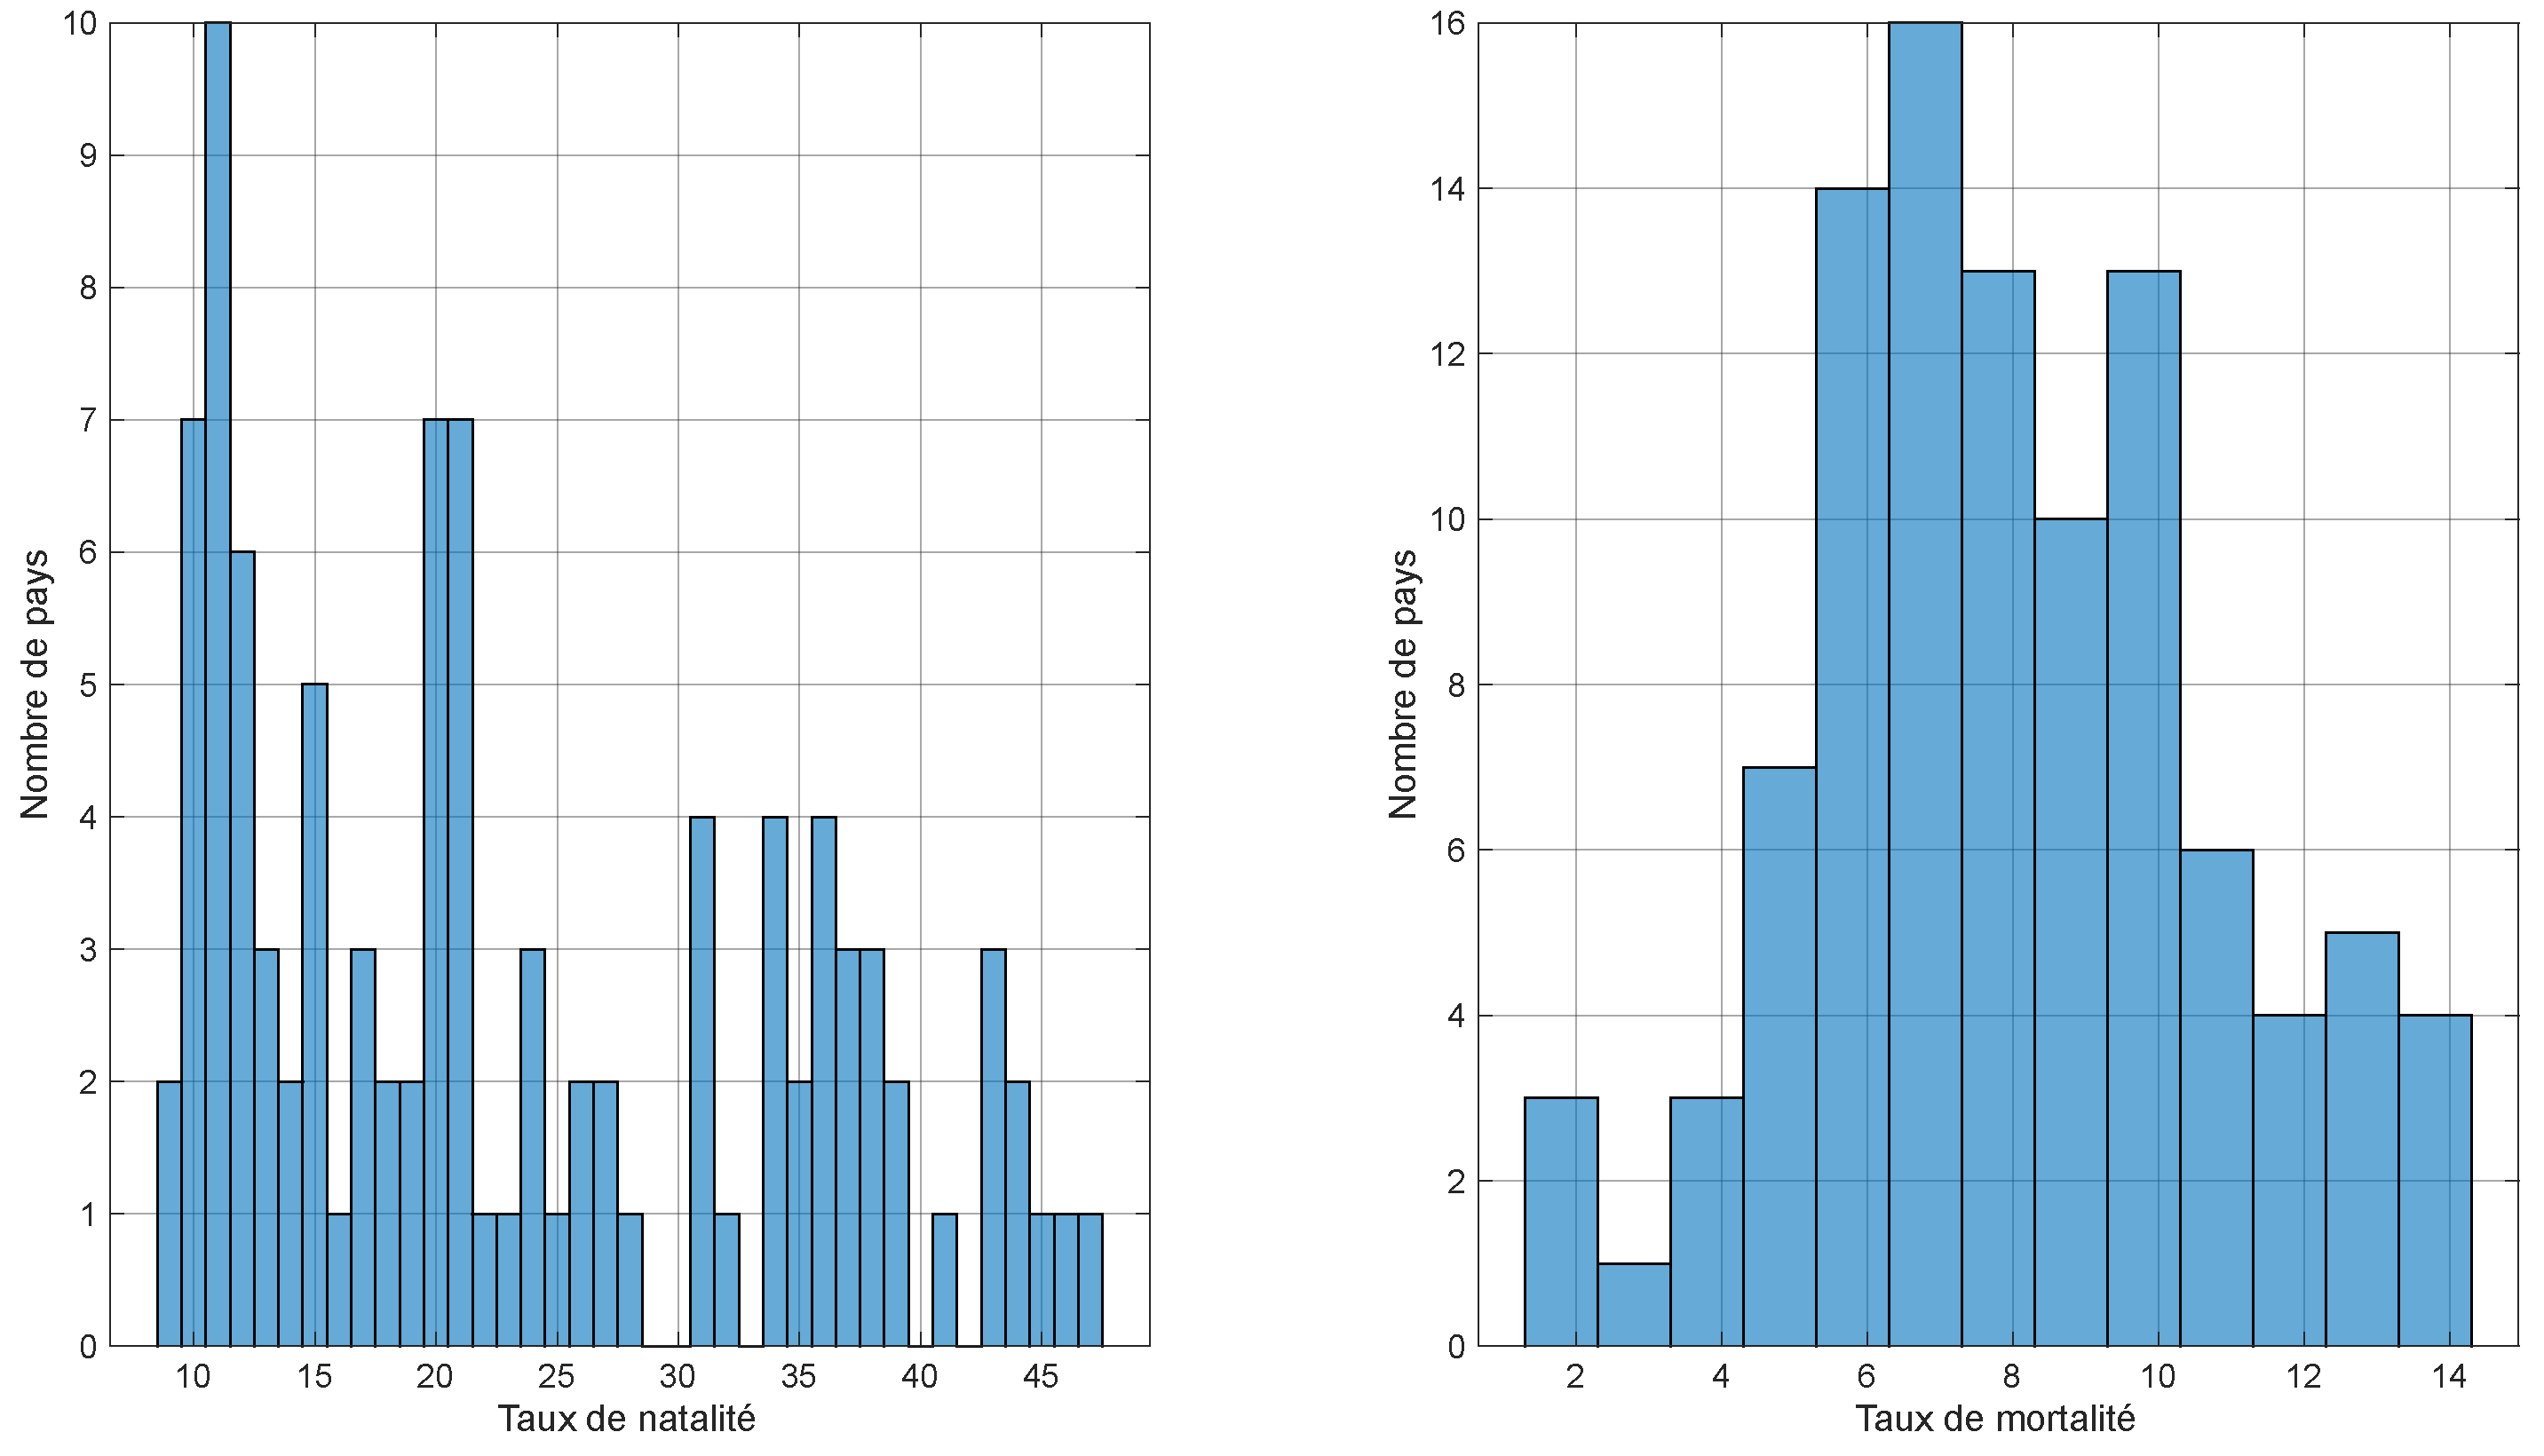
\includegraphics[width=\textwidth]{resources/pdf/figures/Q1a.pdf}
	    \caption{Histogrammes des taux de natalité et de mortalité dans le monde.}
	    \label{fig:Q1a}
	\end{figure}
	
	Il est intéressant de mettre ces deux figures en parallèle afin de constater que le nombre maximum de naissances est largement (environ \num{4} fois) supérieur au nombre maximum de décès, traduisant, d'un point de vue démographique, une augmentation massive de la population mondiale. Une cause possible serait l'évolution technologique et qualitative des soins de santé, permettant à l'Homme de vivre bien plus longtemps qu'auparavant.
	
	% Question 1 - b)
	\subsection{Statistiques descriptives des taux mondiaux}
	\label{subsec:Q1b}
	Les statistiques descriptives des taux mondiaux ont été calculées via le script \hyperref[subsec:code-Q1]{\texttt{Q1b}} avec les fonctions \texttt{mean}, \texttt{median}, \texttt{mode} et \texttt{std}\footnote{Sauf indication contraire, tous les écarts-types calculés sont les écarts-types classiques, issus des variances non corrigées.} et sont présentées dans la table \ref{tab:Q1b}.\par
	
	On remarque que pour le taux de natalité, la moyenne et la médiane sont un peu distantes l'une de l'autre et toutes deux distante du mode, confirmant cette répartition éparse observée à la section \ref{subsec:Q1a}.\par
	
	Ces 3 valeurs, pour le taux de mortalité, sont au contraire assez proches l'une de l'autre. L'écart-type du taux de mortalité est relativement faible, contrairement à celui du taux de natalité qui assez élevé, traduisant une fois de plus l'étalement des données autour de la moyenne.\par
	
	\begin{table}[!ht]
	    \centering
	    \begin{tabular}{|c|c|c|}
	        \hline
	        \textbf{Statistique descriptive} & \textbf{Taux de natalité} & \textbf{Taux de mortalité}\\ \hline
	        \hline
	        Moyenne \(\left [\text{\textperthousand} \right ]\) & \num{23.1510} & \num{8.0270}\\ \hline
	        Médiane  \(\left [\text{\textperthousand} \right ]\) & \num{20.5000} & \num{7.8000}\\ \hline
	        Mode  \(\left [\text{\textperthousand} \right ]\) & \num{11.3000} & \num{9.6000}\\ \hline
	        Écart-type  \(\left [\text{\textperthousand} \right ]\) & \num{11.1497} & \num{2.8567}\\ \hline
	        \hline
	        \textbf{Belgique} & \num{11.7000} & \num{9.9000}\\ \hline
	    \end{tabular}
	    \caption{Statistiques descriptives des taux mondiaux.}
	    \label{tab:Q1b}
	\end{table}
	
	La Belgique présente un taux de natalité largement inférieur à la moyenne mondiale et un taux de mortalité, quant à lui, légèrement supérieur. Le taux de natalité faible s'explique en partie par le fait que la Belgique soit un pays développé, présentant souvent un nombre de naissance compensant à peine le nombre de décès. On peut également remarquer qu'elle est proche du mode du tableau pour les deux taux, signifiant que ce type de proportion est courante dans le monde.
	
	% Question 1 - c)
	\subsection{Caractéristiques d'un taux normal}
	Un taux normal, au sens de la loi normale, est un taux qui est compris dans l'intervalle
	\begin{displaymath}
	    \left [\mu - \sigma; \mu + \sigma \right ]
	\end{displaymath}
	avec
	
	\begin{itemize}
	    \item \(\mu\), la moyenne de la population;
	    \item \(\sigma\), l'écart-type de la population.
	\end{itemize}
	
	Ces deux valeurs ayant été calculées à la section \ref{subsec:Q1b}, le script \hyperref[subsec:code-Q1]{\texttt{Q1c}} détermine l'intervalle pour chaque taux. Ceux-ci sont présentés à la table \ref{tab:Q1c}.\par
	
	\begin{table}[!ht]
	    \centering
	    \begin{tabular}{|c|c|c|}
	        \hline
	        \textbf{Taux} & \textbf{Intervalle} \(\left [\text{\textperthousand} \right ]\)\\ \hline
	        \hline
	        Taux de natalité & \(\left [\num{12.0013}; \num{34.3007} \right]\)\\ \hline
	        Taux de mortalité & \(\left [\num{5.1703}; \num{10.8837} \right]\)\\ \hline
	    \end{tabular}
	    \caption{Intervalles des taux normaux (au sens de la loi normale).}
	    \label{tab:Q1c}
	\end{table}
	
	Le script \hyperref[subsec:code-Q1]{\texttt{Q1c}} calcule également que 54\% des pays ont un taux de natalité normal et 68\% un taux de mortalité normal.\par
	
	Le taux de natalité prenant des valeurs très étendues avec une répartition éparse comme visible sur l'histogramme, il est donc logique que la proportion associée soit importante mais pas très élevée. À l'opposé, les valeurs du taux de mortalité étant déjà approximativement concentrées autour de leur moyenne, son histogramme se rapprochait déjà de la loi normale et la proportion de pays appartenant à l'intervalle est directement plus grande.\par
	
	Concernant la Belgique, son taux de natalité se situe à gauche de l'intervalle des taux normaux et son taux de mortalité se situe dans l'intervalle. Son taux de natalité n'est donc pas normal au sens de la loi normale, mais bien son taux de mortalité. 
	
	% Question 1 - d)
	\subsection{Boîtes à moustaches}
	Les boîtes à moustaches des taux de natalité et de mortalité, générées par le script \hyperref[subsec:code-Q1]{\texttt{Q1d}} avec la fonction \texttt{boxplot}, sont présentées à la figure \ref{fig:Q1d}.\par
	
	\begin{figure}[!ht]
	    \centering
	    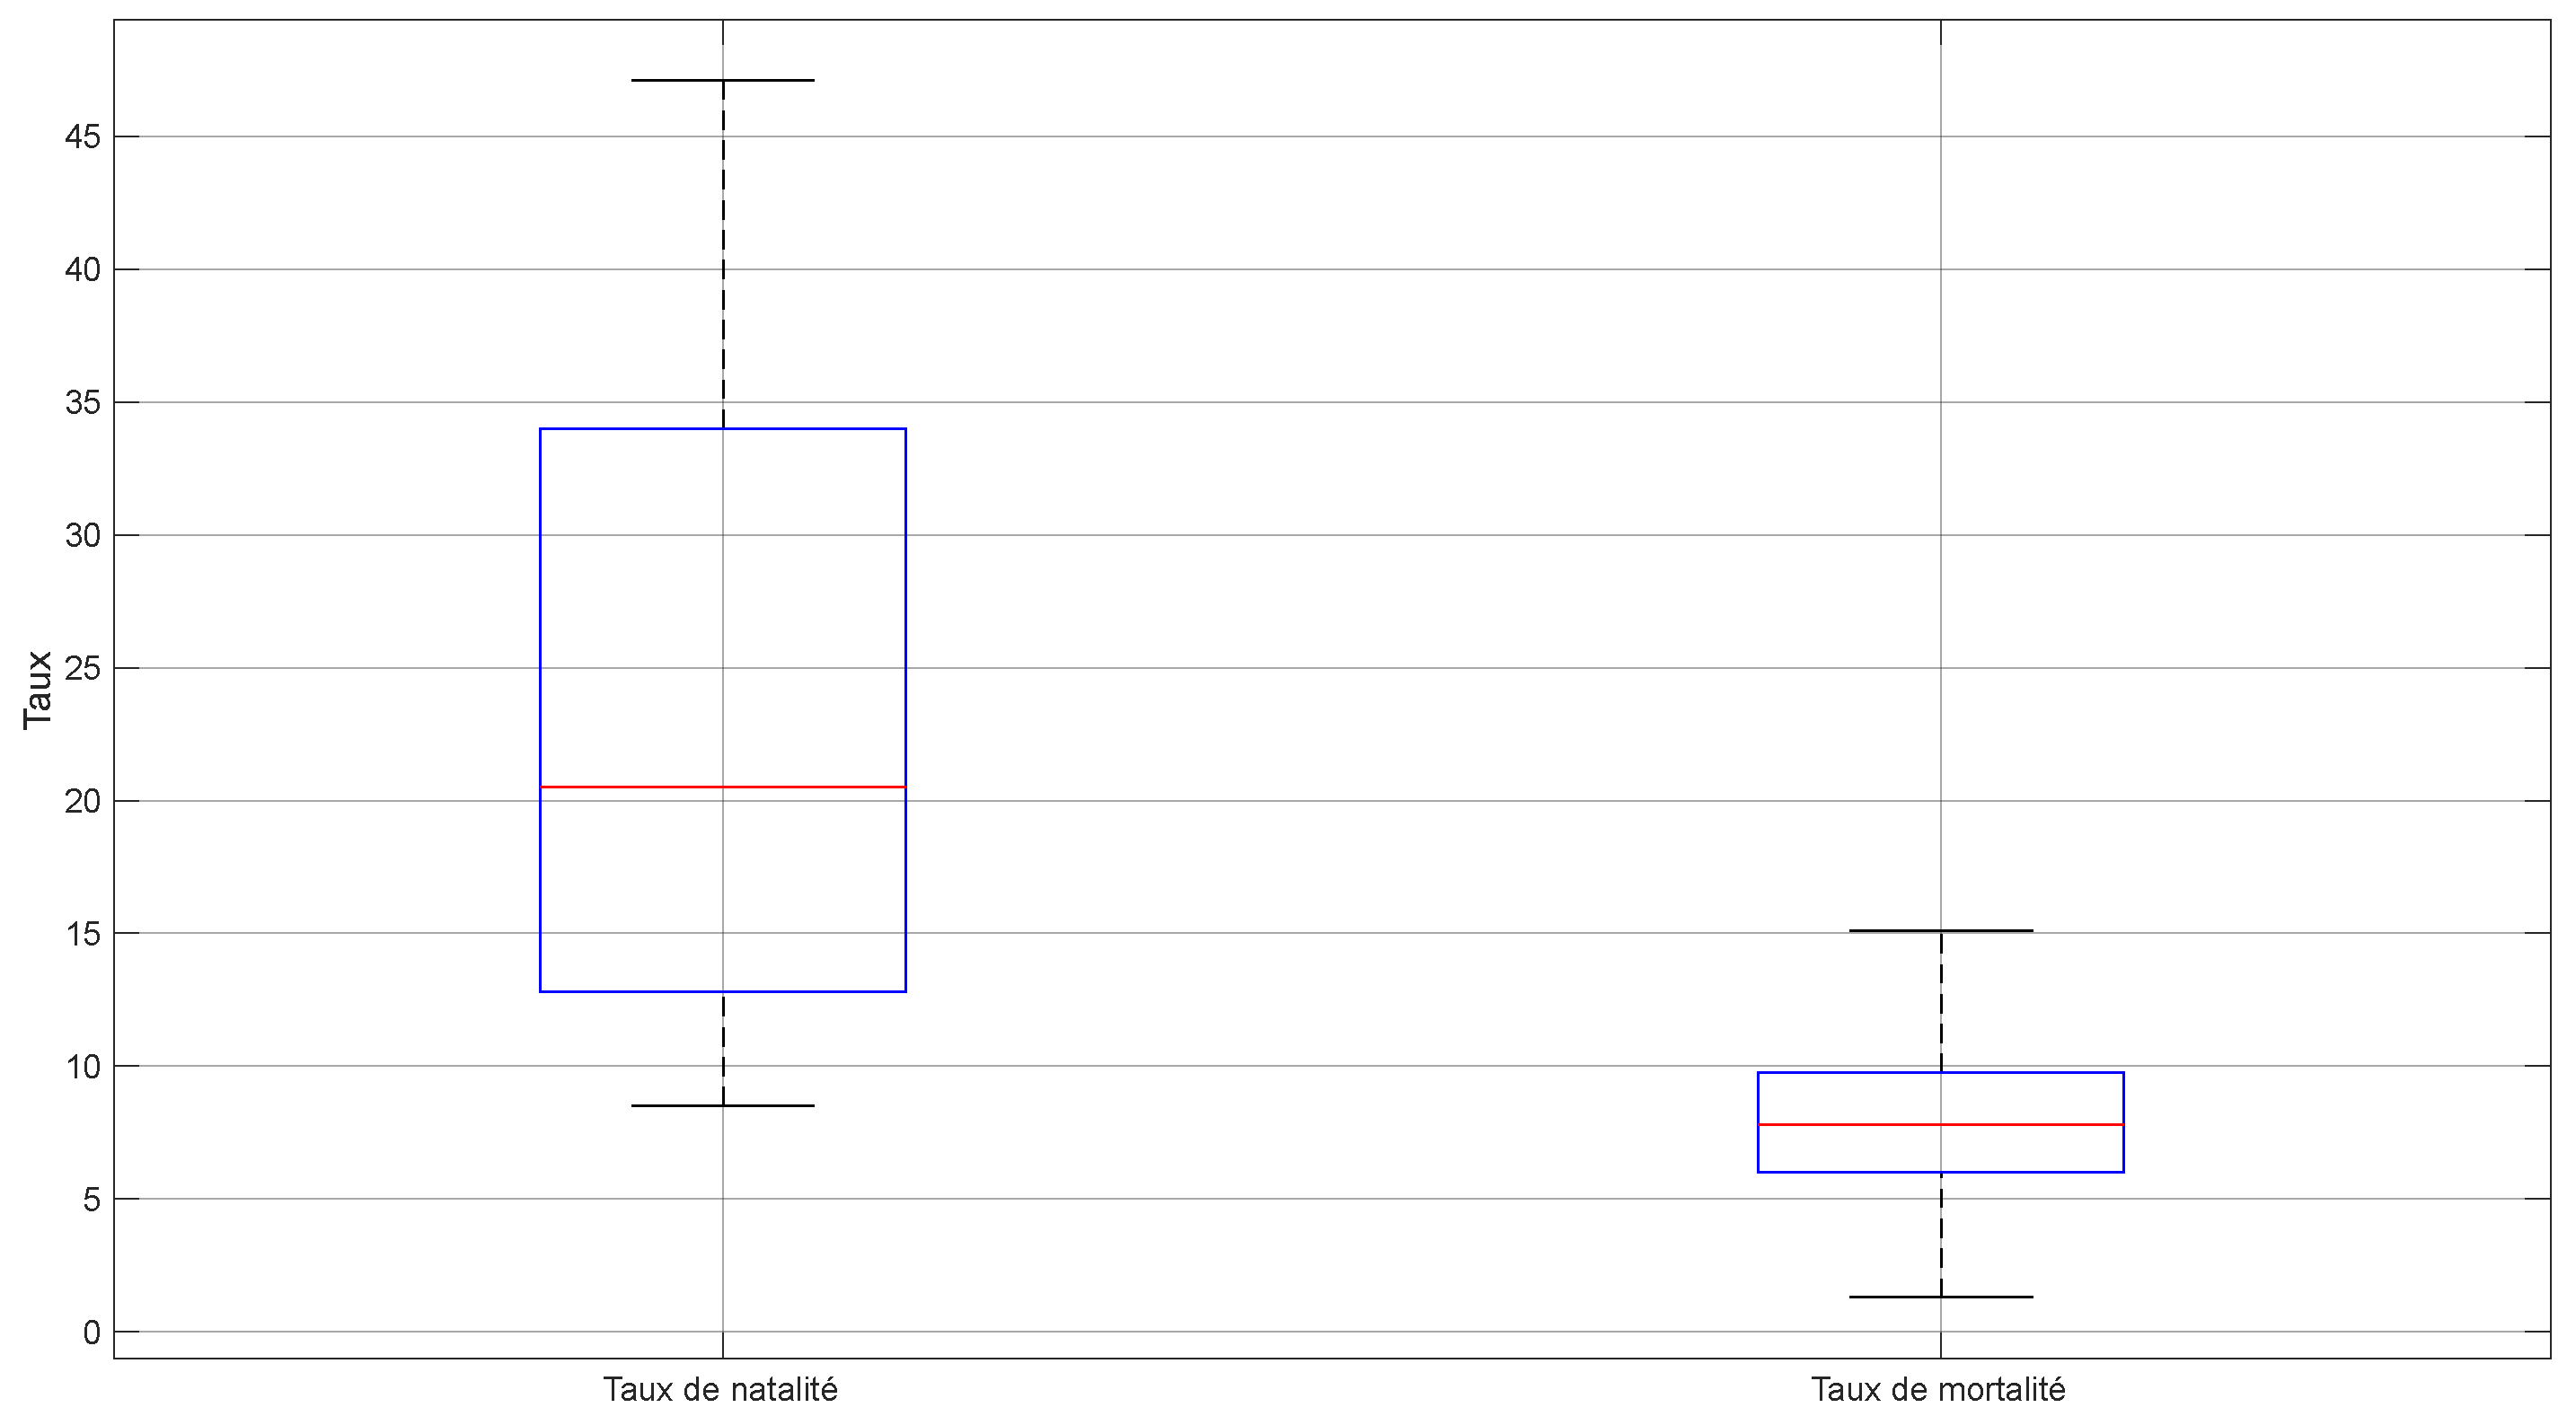
\includegraphics[width=\textwidth]{resources/pdf/figures/Q1d.pdf}
	    \caption{Boîtes à moustaches relatives aux taux de natalité et de mortalité.}
	    \label{fig:Q1d}
	\end{figure}
	
	On constate immédiatement l'absence de données aberrantes pour les deux taux (aucun symbole \og \textcolor{red}{+}\fg{} sur les figures, confirmé également par le script). Les quartiles, calculés avec la fonction \texttt{prctile}, sont explicités à la table \ref{tab:Q1d}. À noter que les deuxièmes quartiles, en rouge sur les boîtes à moustaches, sont les médianes, déjà calculées à la section \ref{subsec:Q1b}.\par
	
	\begin{table}[!ht]
	    \centering
	    \begin{tabular}{|c|c|c|}
	        \hline
	        \textbf{Taux} & \textbf{Premier quartile} \(\left [\text{\textperthousand} \right ]\) & \textbf{Troisième quartile} \(\left [\text{\textperthousand} \right ]\)\\ \hline
	        \hline
	        Taux de natalité & \num{12.8000} & \num{34.0000}\\ \hline
	        Taux de mortalité & \num{6.0000} & \num{9.7500}\\ \hline
	    \end{tabular}
	    \caption{Quartiles du taux de natalité et de mortalité.}
	    \label{tab:Q1d}
	\end{table}
	
	On constate que les deux quartiles concernant le taux de natalité sont fort écartés, reprenant donc un grand nombre de pays dans la boîte, tandis que celle du taux de mortalité voit ses quartiles être très resserrés autour de la valeur médiane. Concernant les moustaches, appelées également bornes aberrantes, celles de la natalité sont asymétriques et la valeur maximale est très élevée, alors que celles du taux de mortalité sont symétriques par rapport à la médiane, traduisant une nouvelle fois l'allure de gaussienne de son histogramme.
	
	% Question 1 - e)
	\subsection{Polygone des fréquences cumulées du taux de natalité}
	Le polygone des fréquences cumulées du taux de natalité, généré par le script \hyperref[subsec:code-Q1]{\texttt{Q1e}} via la fonction \texttt{cdfplot}, est présenté à la figure \ref{fig:Q1e}.\par
	
	\begin{figure}[!ht]
	    \centering
	    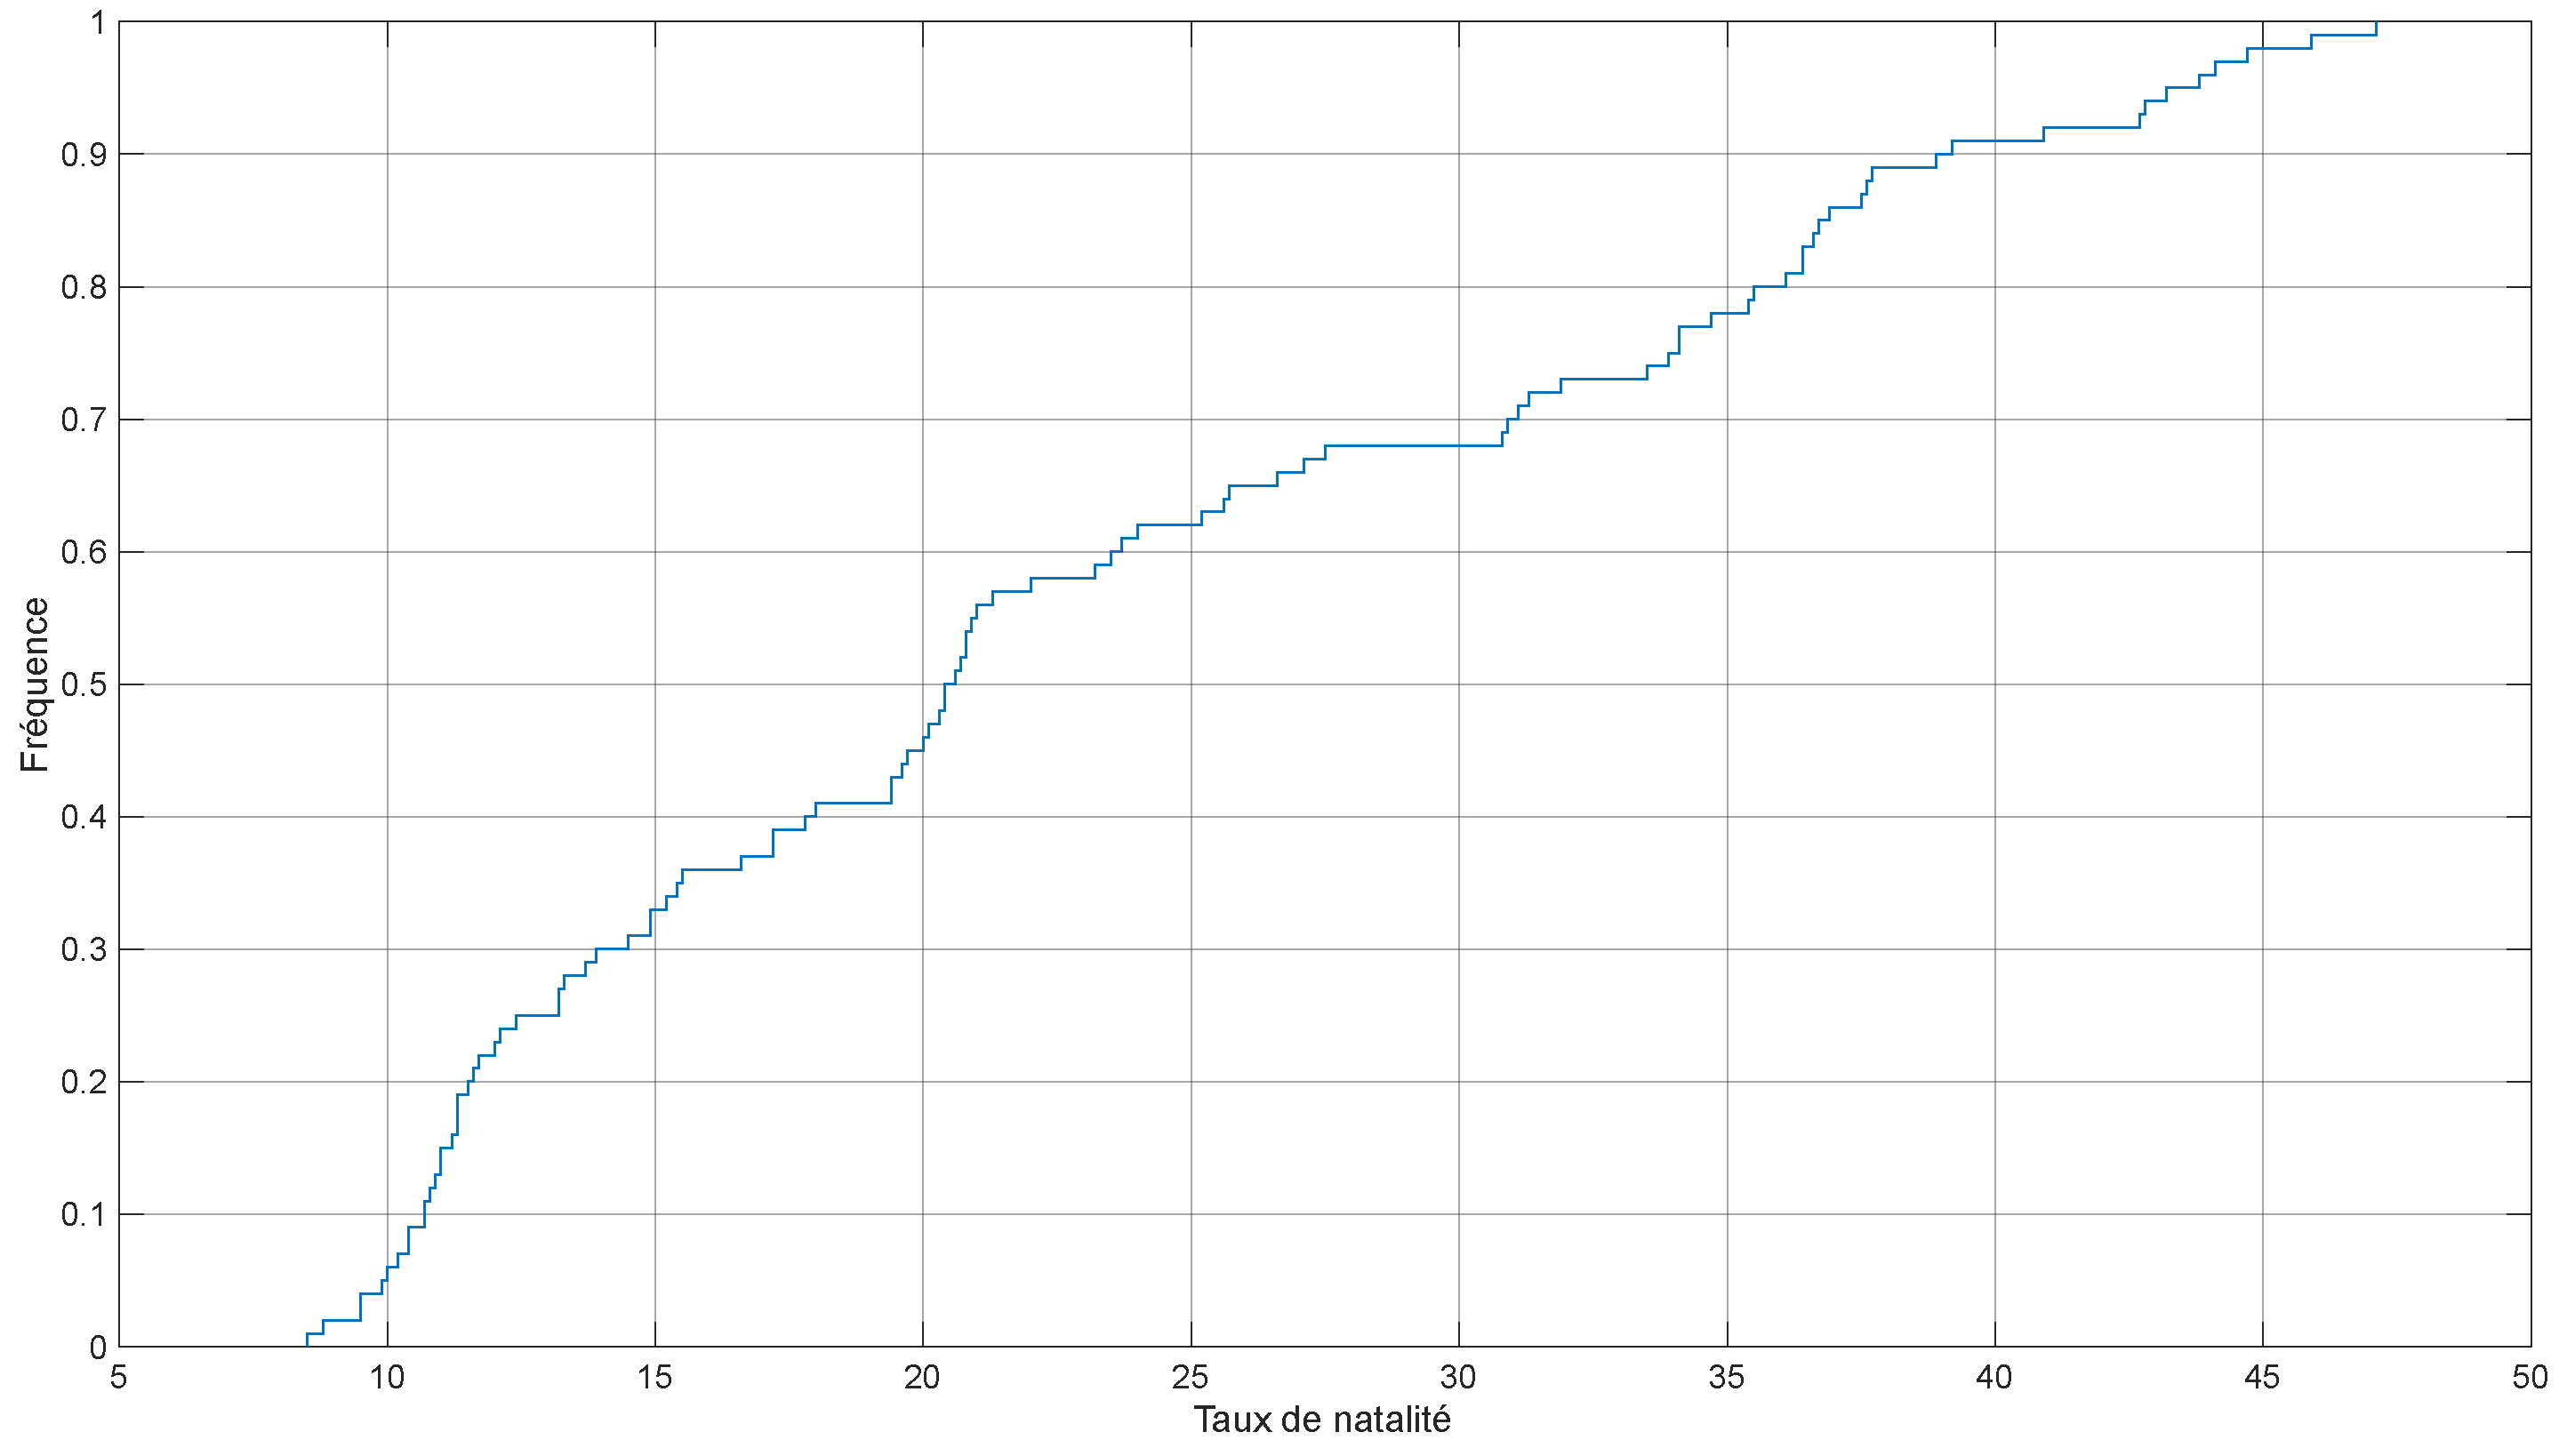
\includegraphics[width=\textwidth]{resources/pdf/figures/Q1e.pdf}
	    \caption{Polygone des fréquences cumulées du taux de natalité.}
	    \label{fig:Q1e}
	\end{figure}
	
	L'estimation de la proportion de pays ayant un taux de natalité inférieur ou égal à \num{20} pour \num{1000} habitants et supérieur à celui de la Belgique est donnée par
	\begin{align*}
	    F\left (\num{20}\right ) - F\left (\num{11.7}\right ) &= \num{0.4600} - \num{0.2200}\\
	    &= \num{0.2400}
	\end{align*}
	En effet, la valeur du polygone au point \(x = \num{20}\) (\(F\left (\num{20}\right )\), calculée avec la fonction \texttt{ecdf}) donne la proportion de pays ayant un taux de natalité inférieur ou égal à \num{20}. En retirant à cette proportion celle des pays ayant un taux de natalité inférieur ou égal à celui de la Belgique (\(F\left (\num{11.7}\right )\)), on obtient bien la proportion de pays appartenant à l'intervalle demandé.
	
	% Question 1 - f)
	\subsection{Nuage de points}
	Le nuage de points (\textit{scatterplot}) comparant les deux taux, généré par la fonction \texttt{scatter} du script \hyperref[subsec:code-Q1]{\texttt{Q1f}}, est présenté à la figure \ref{fig:Q1f}.\par
	
	\begin{figure}[!ht]
	    \centering
	    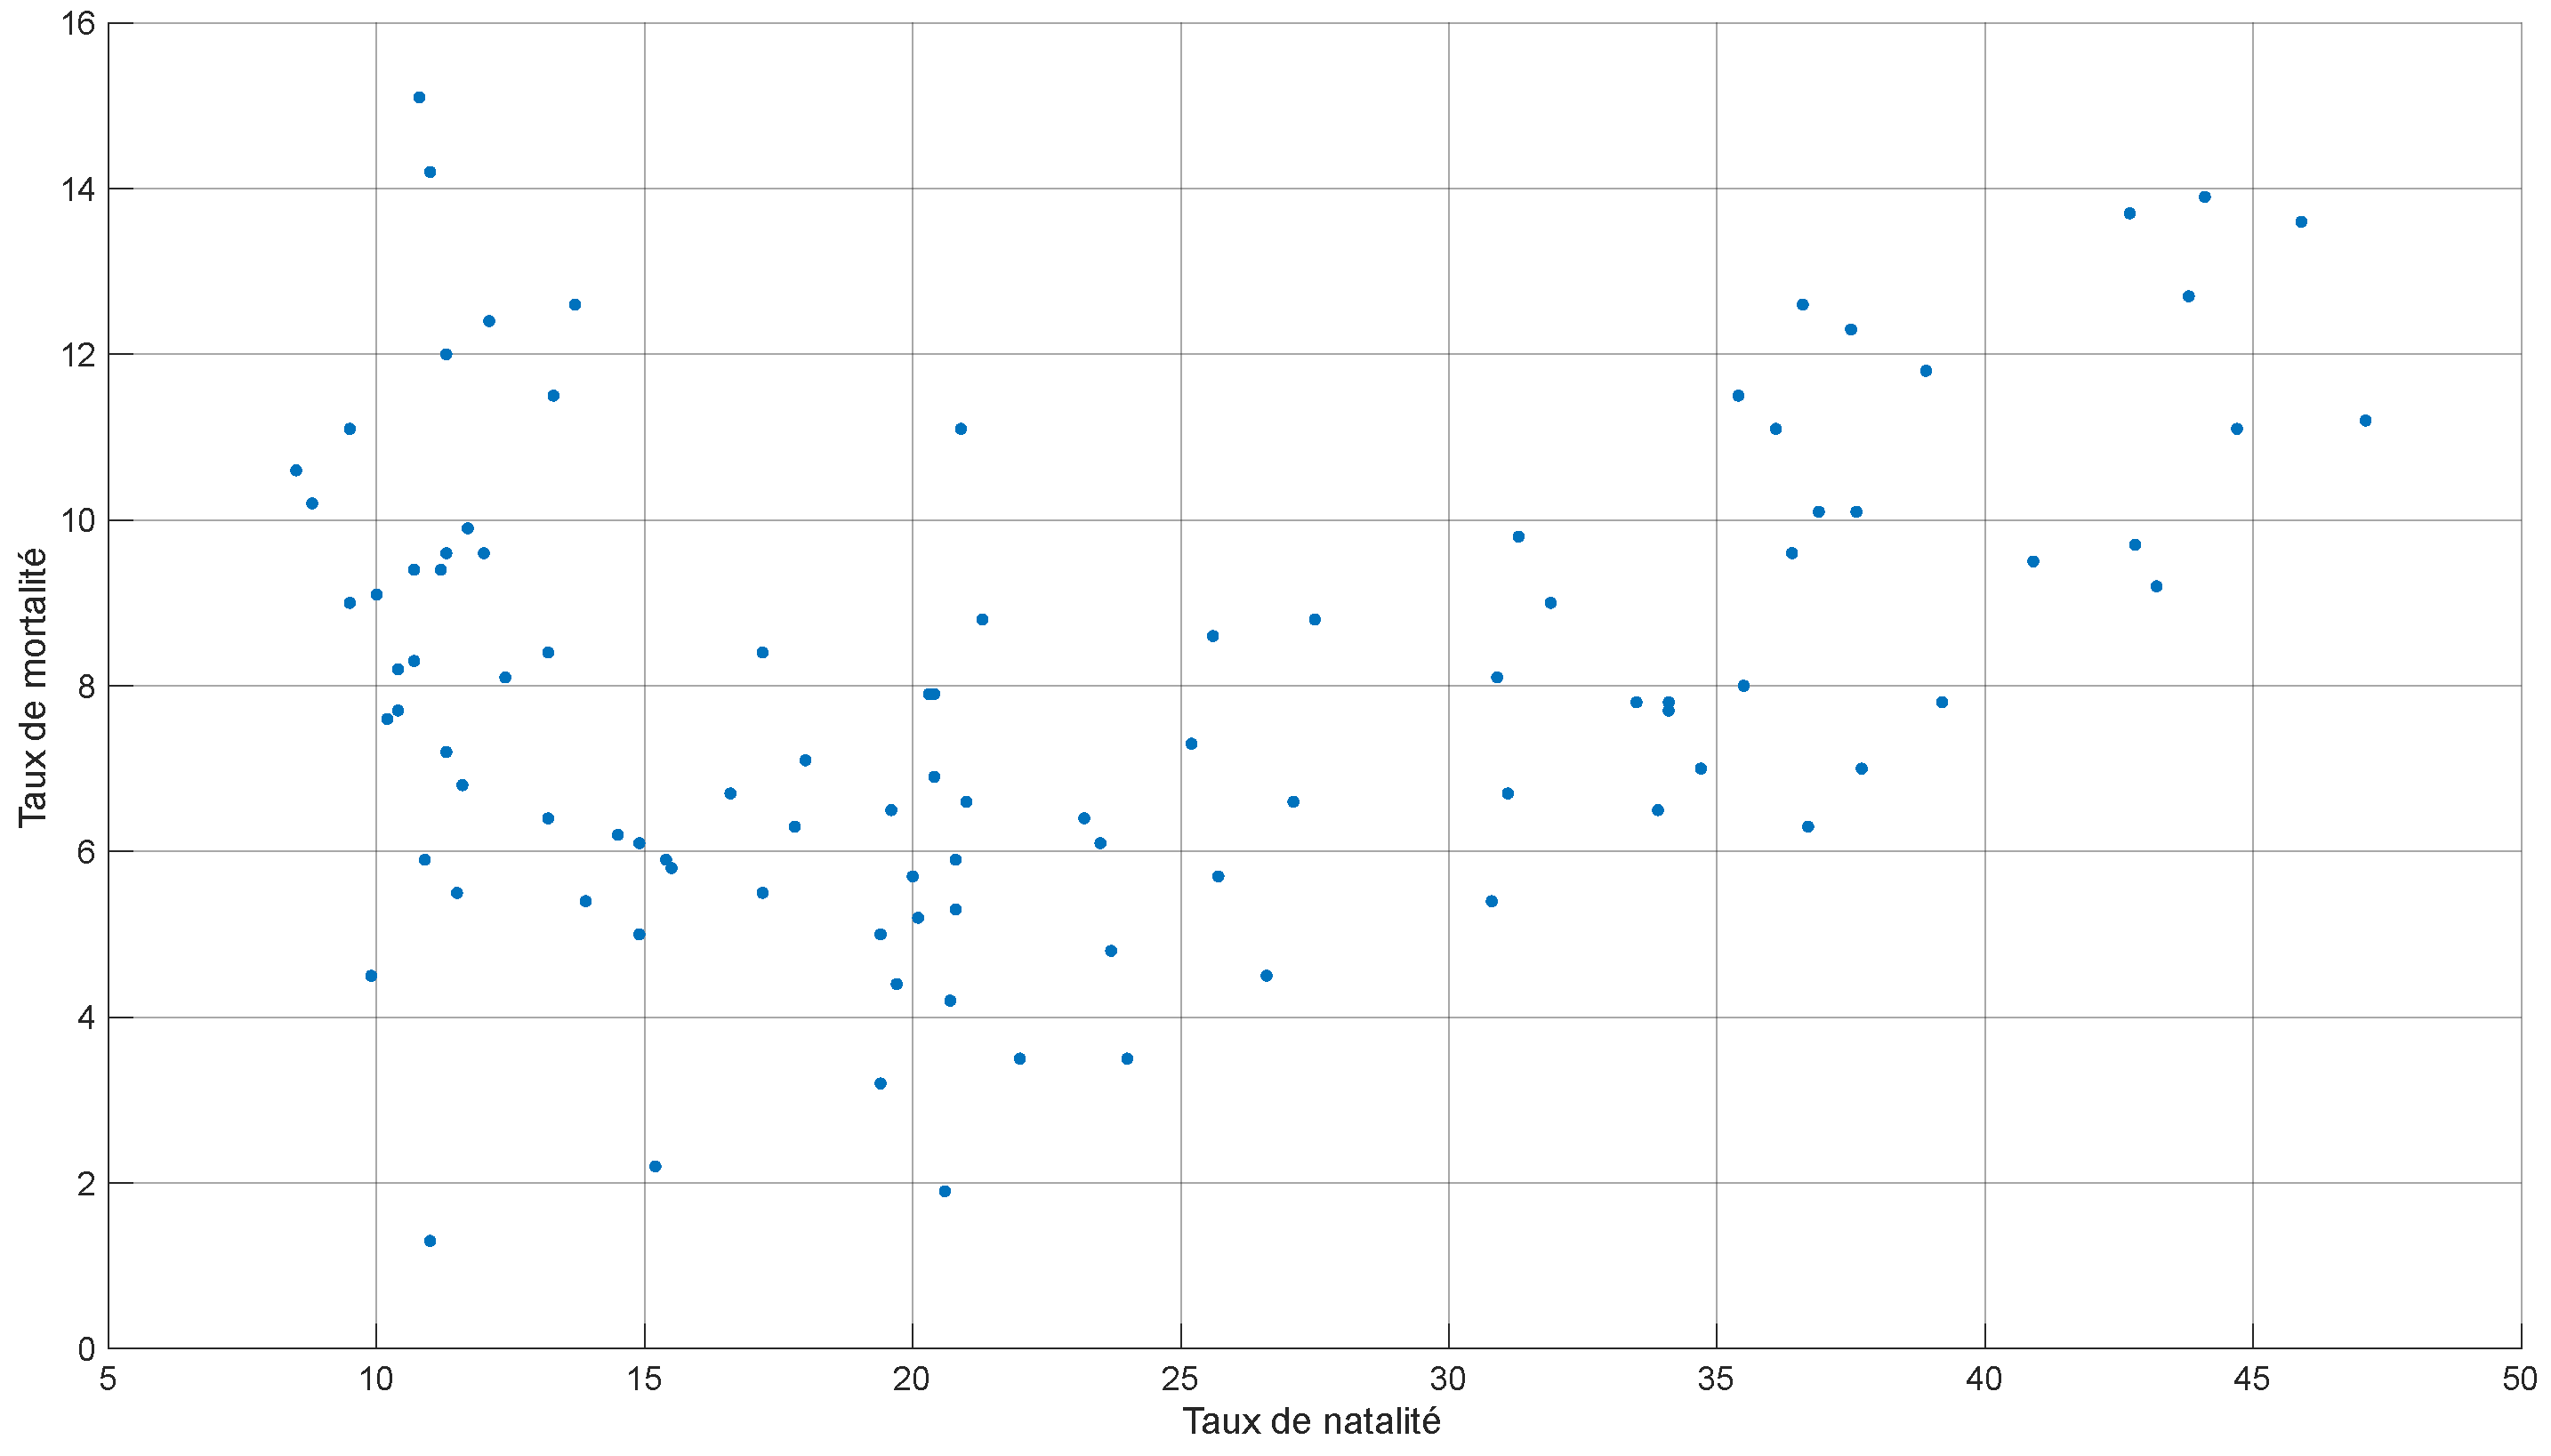
\includegraphics[width=\textwidth]{resources/pdf/figures/Q1f.pdf}
	    \caption{Nuage de points corrélant le taux de natalité et le taux de mortalité.}
	    \label{fig:Q1f}
	\end{figure}
	
	Il est difficile de tirer une relation entre les deux taux sur base de cette figure. On constate tout de même que les pays ayant un taux de natalité élevé ont également tendance à avoir un taux de mortalité élevé lui aussi.\par
	
	Le coefficient de corrélation entre le taux de natalité et le taux de mortalité, calculé avec \texttt{corrcoef}, vaut \num{0.2803}. Ces deux taux sont donc faiblement corrélés.\par
	
	
	% ---------- Génération d'échantillons i.i.d. ---------- %
	\section{Génération d'échantillons i.i.d.}
	
	\paragraph{Remarque préliminaire} Dans toutes les sections et sous-sections suivantes concernant des échantillons i.i.d., les résultats présentés sont issus d'un tirage particulier. Ces valeurs peuvent varier en fonction du tirage effectué. Il est à noter également que, pour une cohérence dans la comparaison des résultats, les mêmes échantillons ont été utilisés pour toutes les sections travaillant sur un même tirage.
	
	% Question 2 - a)
	\subsection{Échantillon i.i.d. de 20 pays}
	On tire, grâce à la fonction auxiliaire \hyperref[subsec:code-auxiliary]{\texttt{getsample}}, un échantillon i.i.d. de 20 pays.
	
	\subsubsection{Statistiques descriptives}
	Les résultats, obtenus grâce au script \hyperref[subsec:code-Q2]{\texttt{Q2a}}, sont explicités à la table \ref{tab:Q2ai}.\par
	
	\begin{table}[!ht]
	    \centering
	    \begin{tabular}{|c|c|c|}
	        \hline
	        \textbf{Statistique descriptive} & \textbf{Taux de natalité} & \textbf{Taux de mortalité}\\ \hline
	        \hline
	        Moyenne \(\left [\text{\textperthousand} \right ]\) & \num{21.0500} & \num{8.1450}\\ \hline
	        Médiane \(\left [\text{\textperthousand} \right ]\) & \num{19.7500} & \num{8.1500}\\ \hline
	        Écart-type \(\left [\text{\textperthousand} \right ]\) & \num{11.6061} & \num{2.6541}\\ \hline
	    \end{tabular}
	    \caption{Statistiques descriptives d'un échantillon i.i.d. de 20 pays.}
	    \label{tab:Q2ai}
	\end{table}
	
	En comparant ces valeurs avec celles de la population (table \ref{tab:Q1b}), on constate qu'elles sont plutôt proches l'une de l'autre. Les variations par rapport aux résultats de la population sont encore trop élevées que pour considérer ces valeurs comme précises. Cependant, dans un cadre général, celles-ci permettent de dégager une tendance et sont donc tout à fait acceptables.
	
	\subsubsection{Boîtes à moustaches}
	De manière générale, les boîtes obtenues (présentées à la figure \ref{fig:Q2aii}), via la fonction \texttt{boxplot} du script \hyperref[subsec:code-Q2]{\texttt{Q2a}}, s'apparentent au boîtes à moustaches de la population (figure \ref{fig:Q1d}).\par
	
	\begin{figure}[!ht]
	    \centering
	    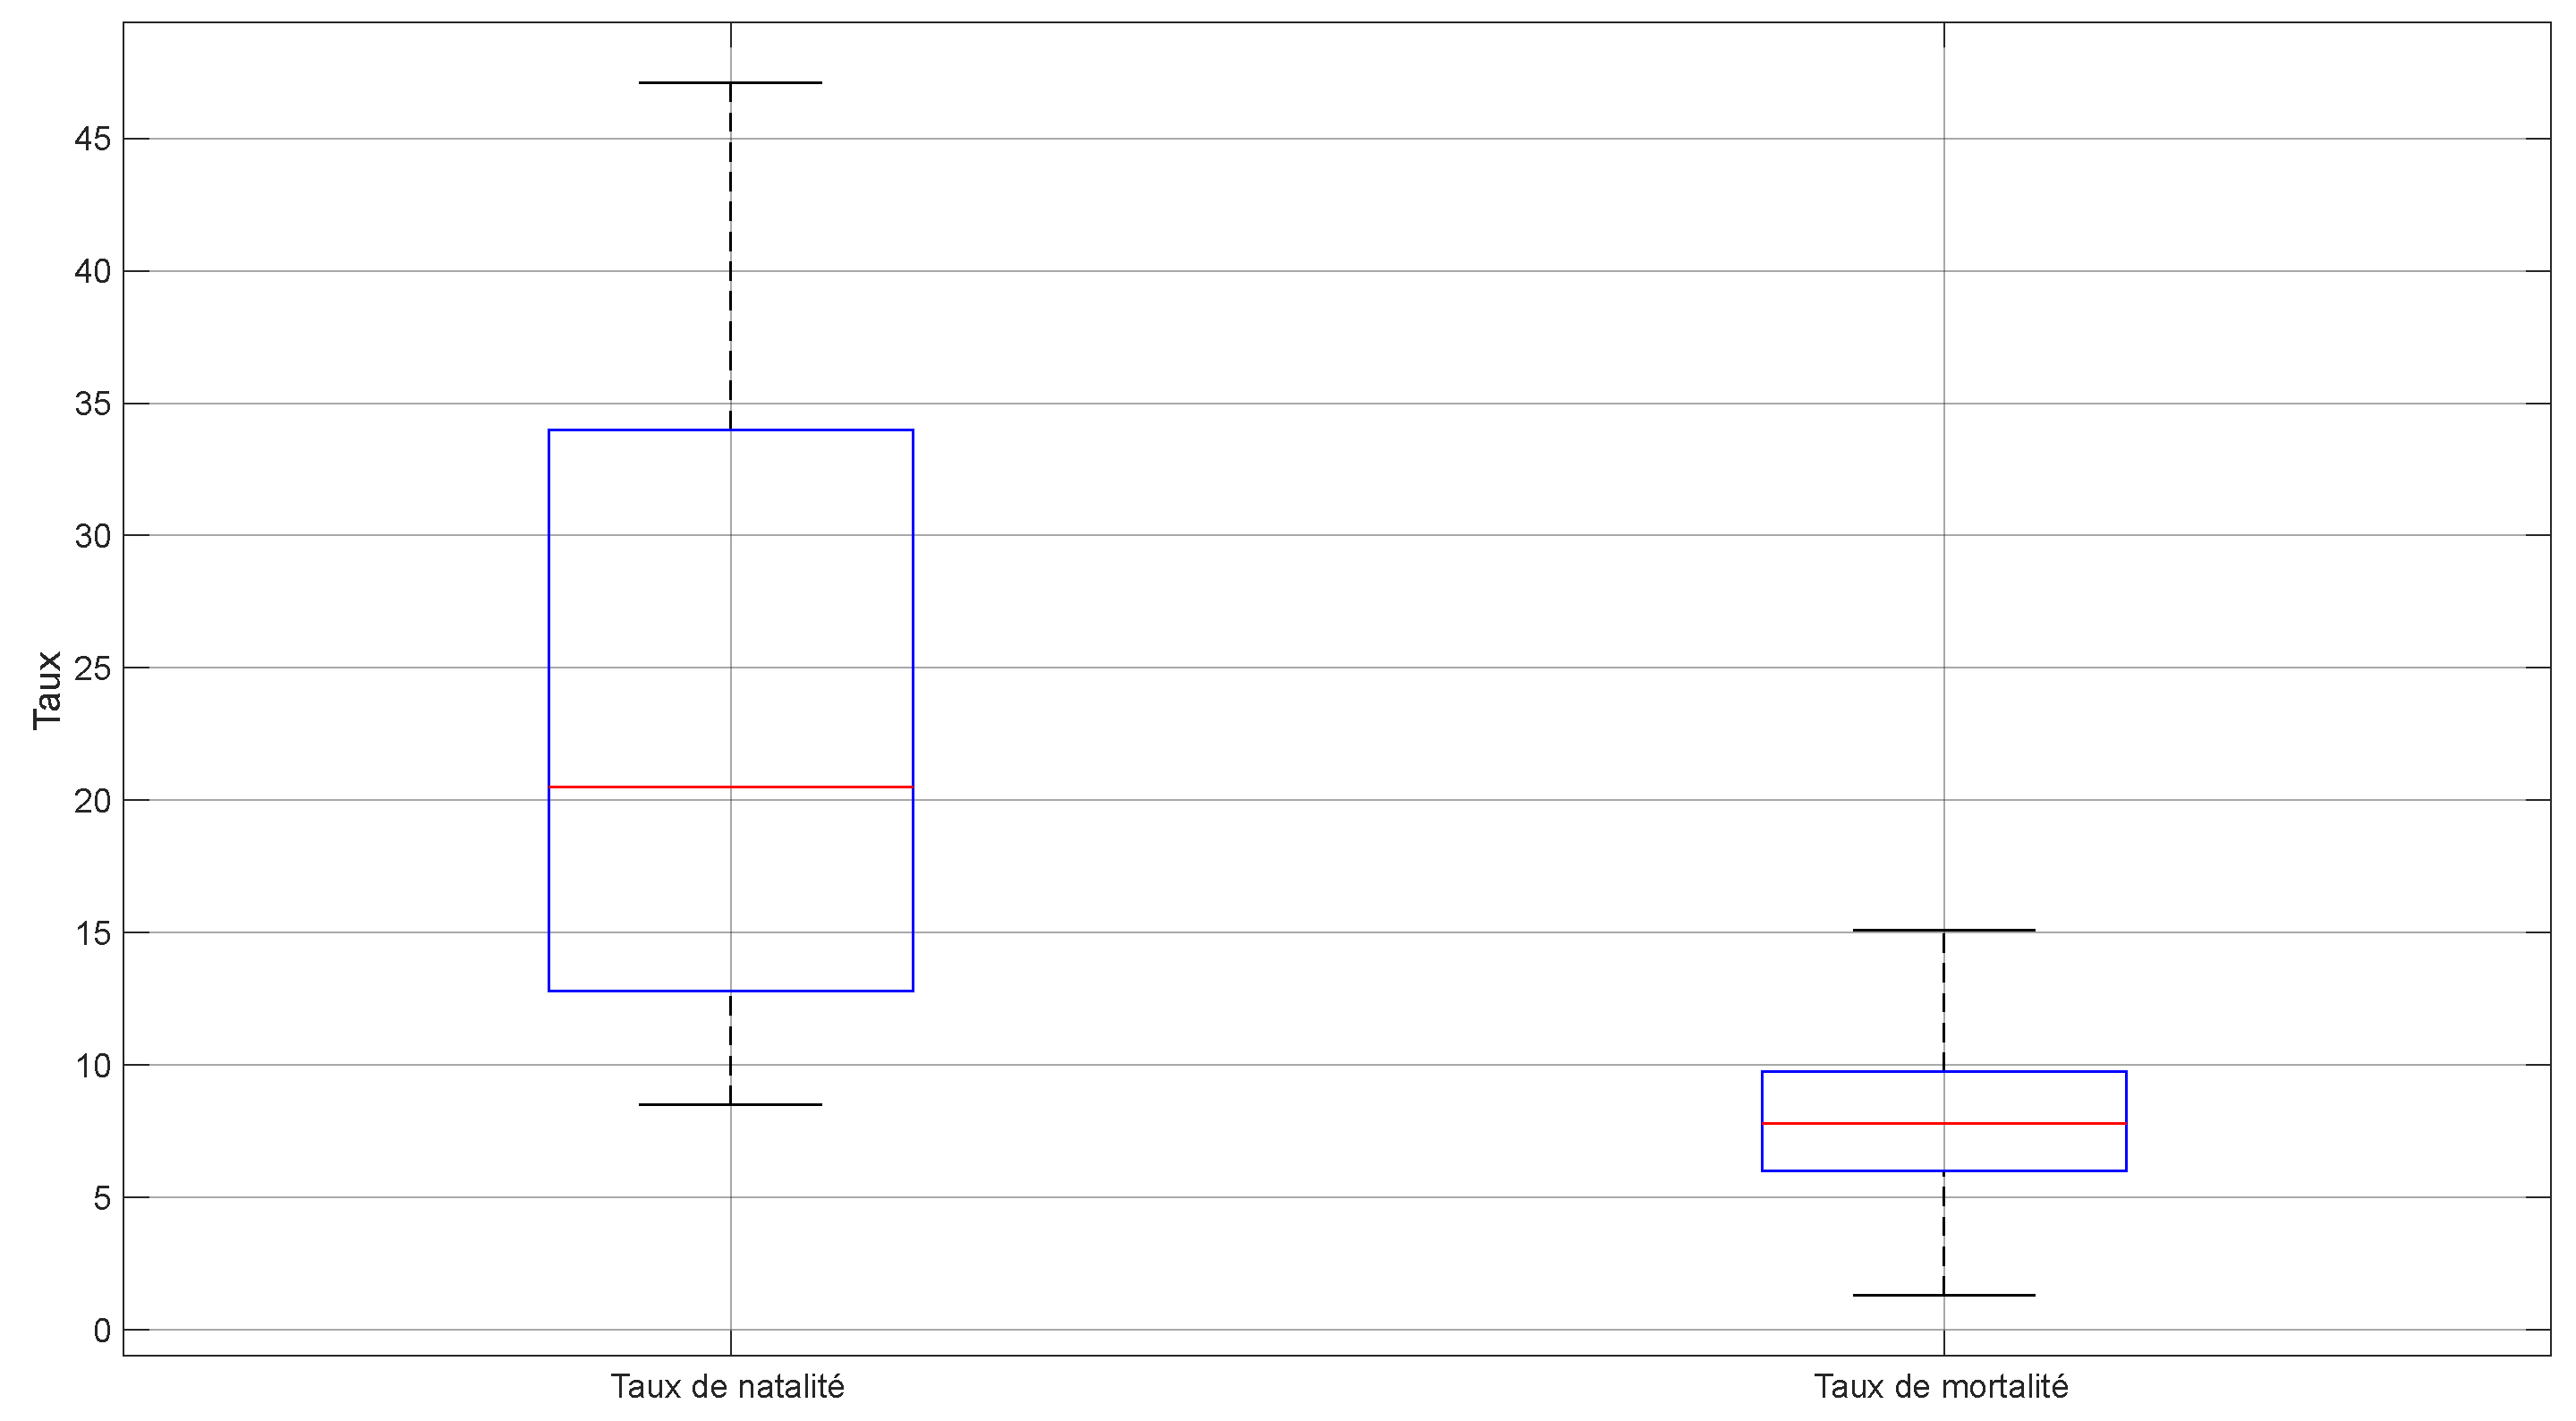
\includegraphics[width=\textwidth]{resources/pdf/figures/Q2aii.pdf}
	    \caption{Boîtes à moustaches d'un échantillon i.i.d. de 20 pays.}
	    \label{fig:Q2aii}
	\end{figure}
	
	La taille de l'échantillon étant assez petite par rapport à la population, il est normal que les valeurs des quartiles varient; surtout celles concernant le taux de natalité dont, de base, les valeurs de la population sont assez éparses. Les moustaches sont, elles aussi, plus restreintes (et seront forcément toujours plus petites ou égales à celle de la population).
	
	\subsubsection{Polygones des fréquences cumulées}
	Les deux graphes des fréquences cumulées, obtenus via le script \hyperref[subsec:code-Q2]{\texttt{Q2a}}, sont présentés à la figure \ref{fig:Q2aiii}.\par
	
	\begin{figure}[!ht]
	    \centering
	    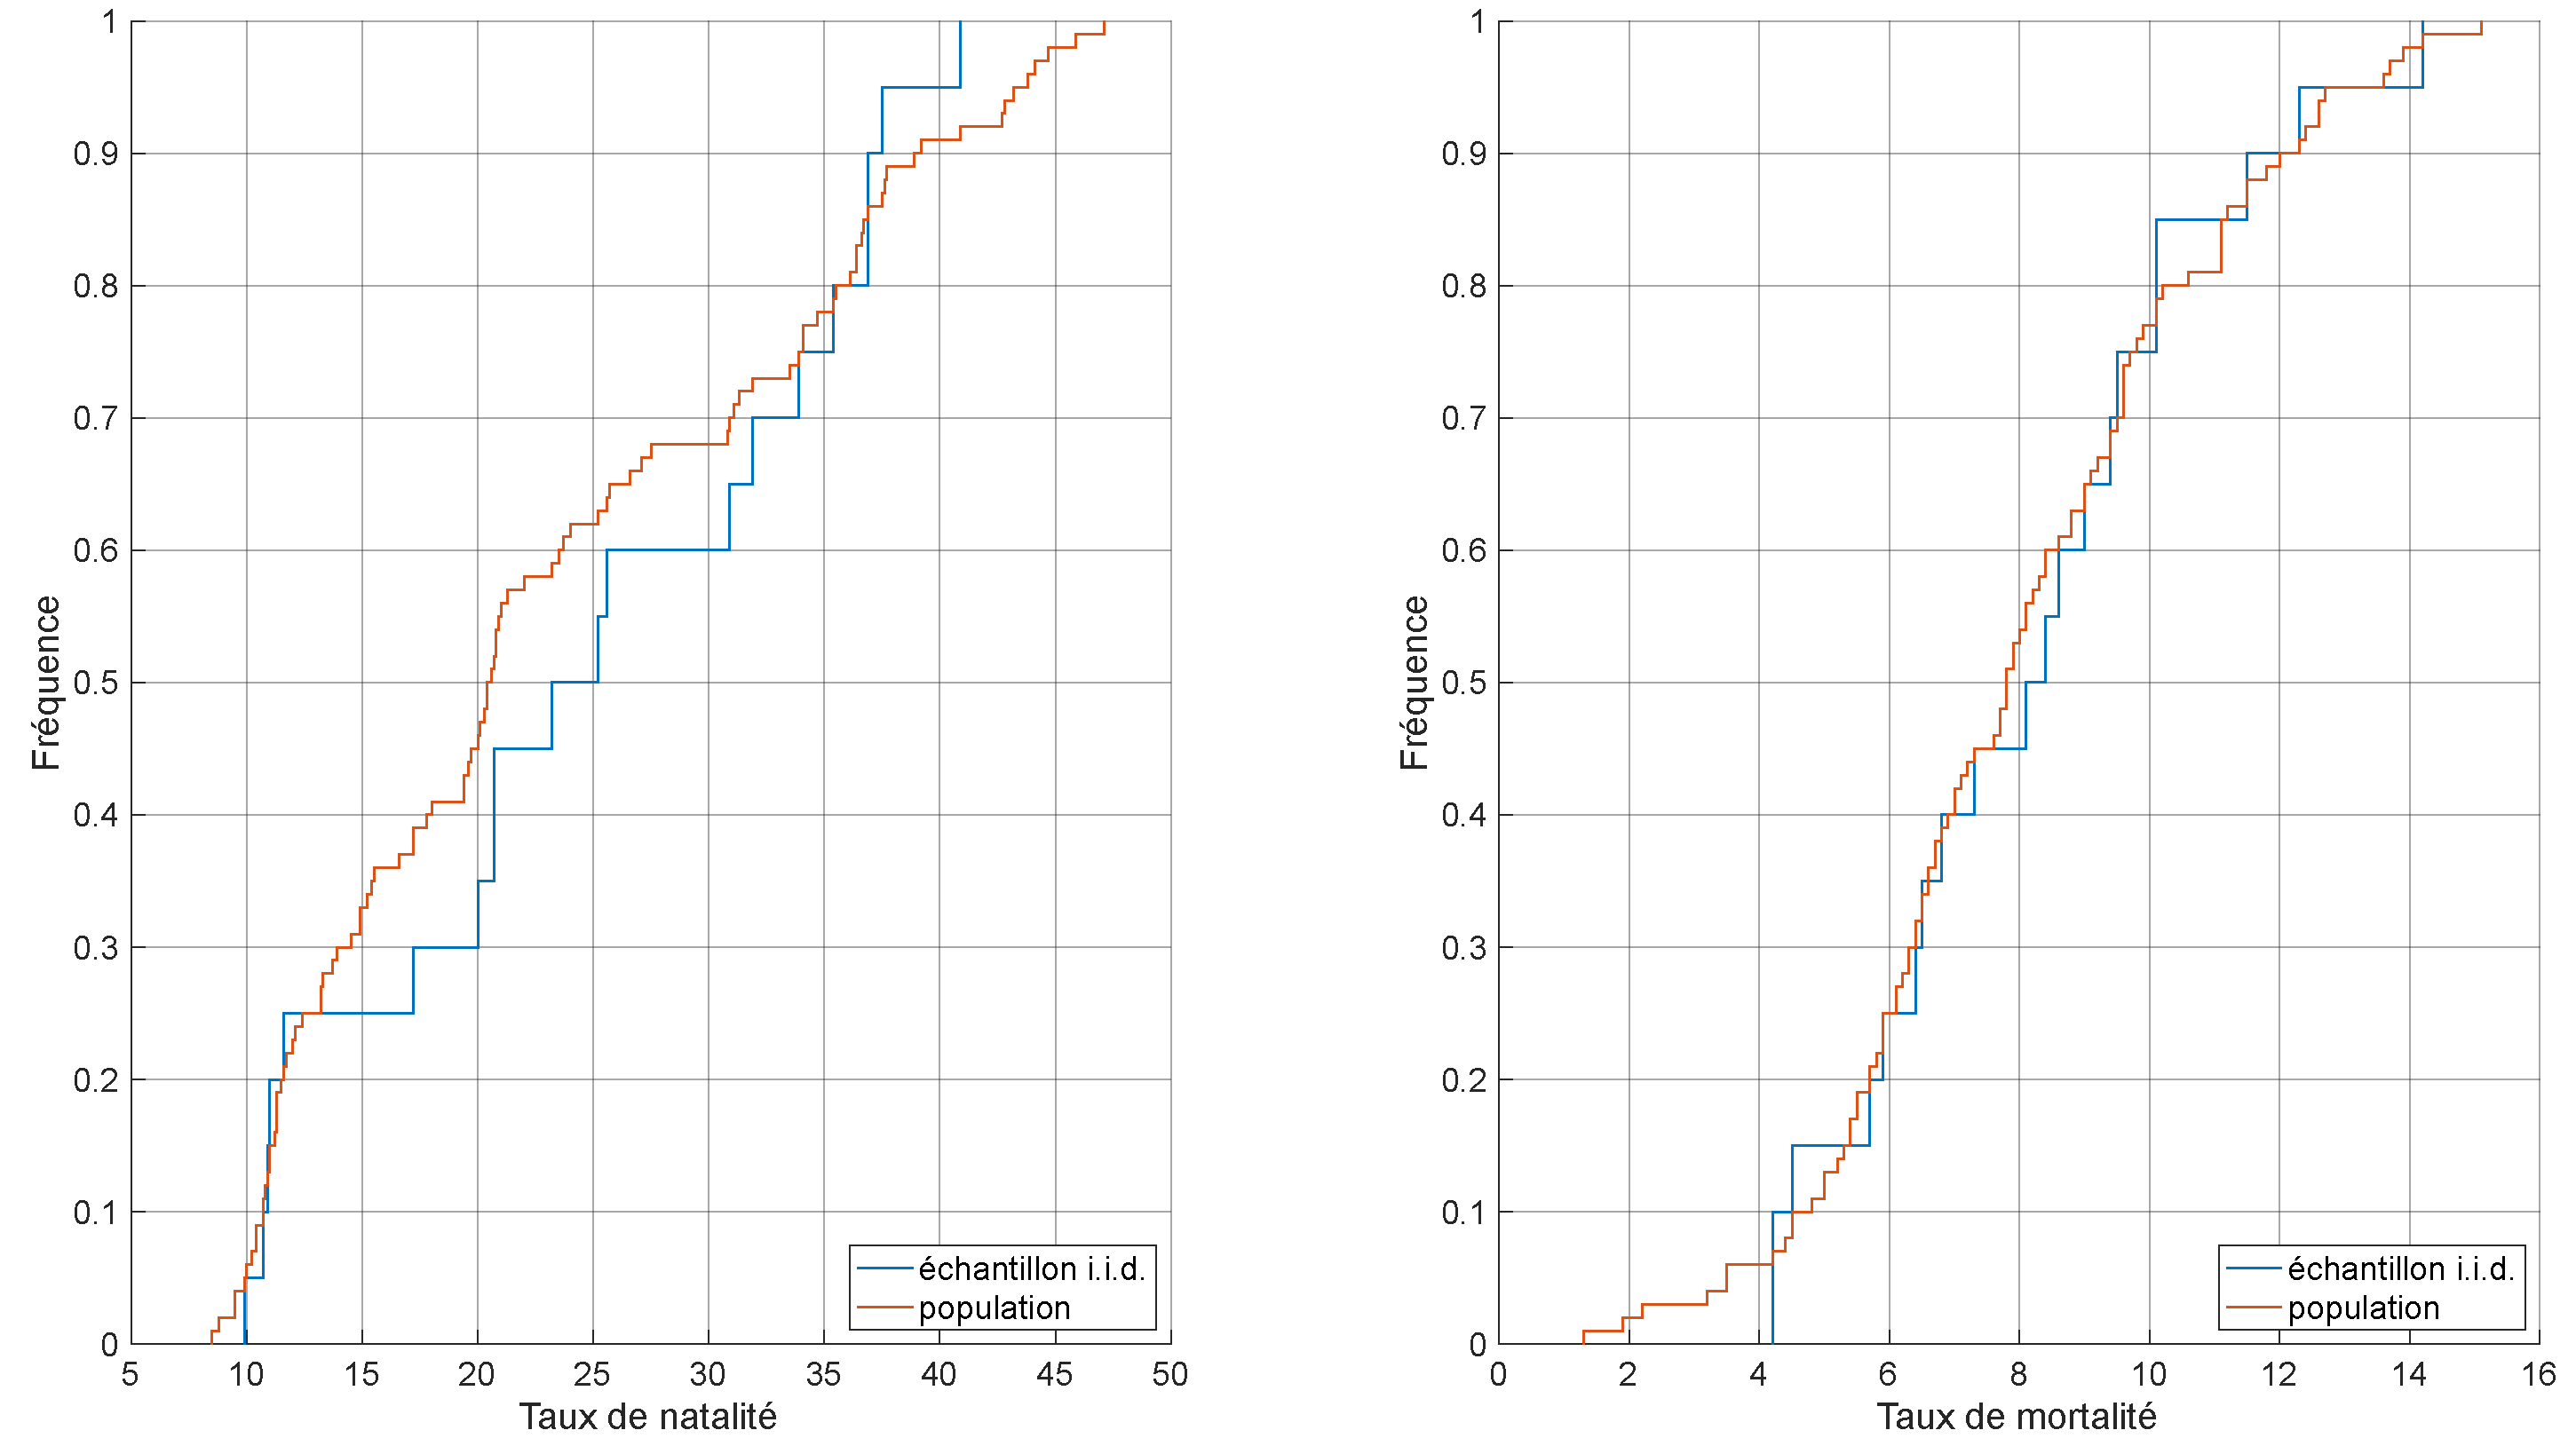
\includegraphics[width=\textwidth]{resources/pdf/figures/Q2aiii.pdf}
	    \caption{Polygones des fréquences cumulées du taux de natalité d'un échantillon i.i.d. de 20 pays.}
	    \label{fig:Q2aiii}
	\end{figure}
	
	Concernant le polygone relatif au taux de natalité, on remarque que l'allure de l'échantillon est relativement semblable à celle de la population. Cependant, le peu de valeur utilisées conduit à un graphe beaucoup moins lisse avec notamment des paliers par endroit. Cette allure dépendra de l'échantillon tiré, notamment pour la présence de paliers, mais conservera la même allure générale.\par
	
	Le polygone du taux de mortalité de l'échantillon est également proche de celui de la population, avec des écarts parfois important, mais qui sont dûs, eux aussi, au nombre de valeurs utilisées.\par
	
	Les deux graphes de l'échantillon se rapprochent donc de ceux de la population mais ne permettent pas de s'en affranchir et de se baser uniquement sur ceux-ci.\par
	
	Les distances de Kolmogorov-Smirnov sont explicitées à la table \ref{tab:Q2aiii}.\par
	
	\begin{table}[!ht]
	    \centering
	    \begin{tabular}{|c|c|}
	        \hline
	        \textbf{Taux} & \textbf{Distance de Kolmogorov-Smirnov}\\ \hline
	        \hline
	        Taux de natalité & \num{0.2400}\\ \hline
	        Taux de mortalité & \num{0.1100}\\ \hline
	    \end{tabular}
	    \caption{Distances de Kolmogorov-Smirnov de l'échantillon i.i.d.}
	    \label{tab:Q2aiii}
	\end{table}
	
	Ces valeurs varient entre \num{0.1500} et \num{0.2500} en fonction du tirage, confirmant ainsi les écarts observables sur la figure \ref{fig:Q2aiii}. On peut noter que ces valeurs ne seront jamais nulles puisqu'un échantillon de \num{20} pays ne coïncidera jamais exactement avec la population de \num{100} pays. Ces distances sont relativement faibles, confirmant ainsi le fait que les résultats de l'échantillons sont acceptables.
	
	% Question 2 - b)
	\subsection{500 échantillons i.i.d. de 20 pays}
	On tire, grâce à la fonction auxiliaire \hyperref[subsec:code-auxiliary]{\texttt{getsample}}, 500 échantillons i.i.d. de 20 pays. Les figures et résultats explicités dans les sous-sections suivantes ont été obtenus par le script \hyperref[subsec:code-Q2]{\texttt{Q2b}}.
	
	\subsubsection{Étude du taux moyen de natalité et de mortalité}
	\label{subsec:Q2bi}
	L'allure des deux histogrammes se rapproche d'une loi normale comme on peut le voir à la figure \ref{fig:Q2bi}.\par
	
	\begin{figure}[!ht]
	    \centering
	    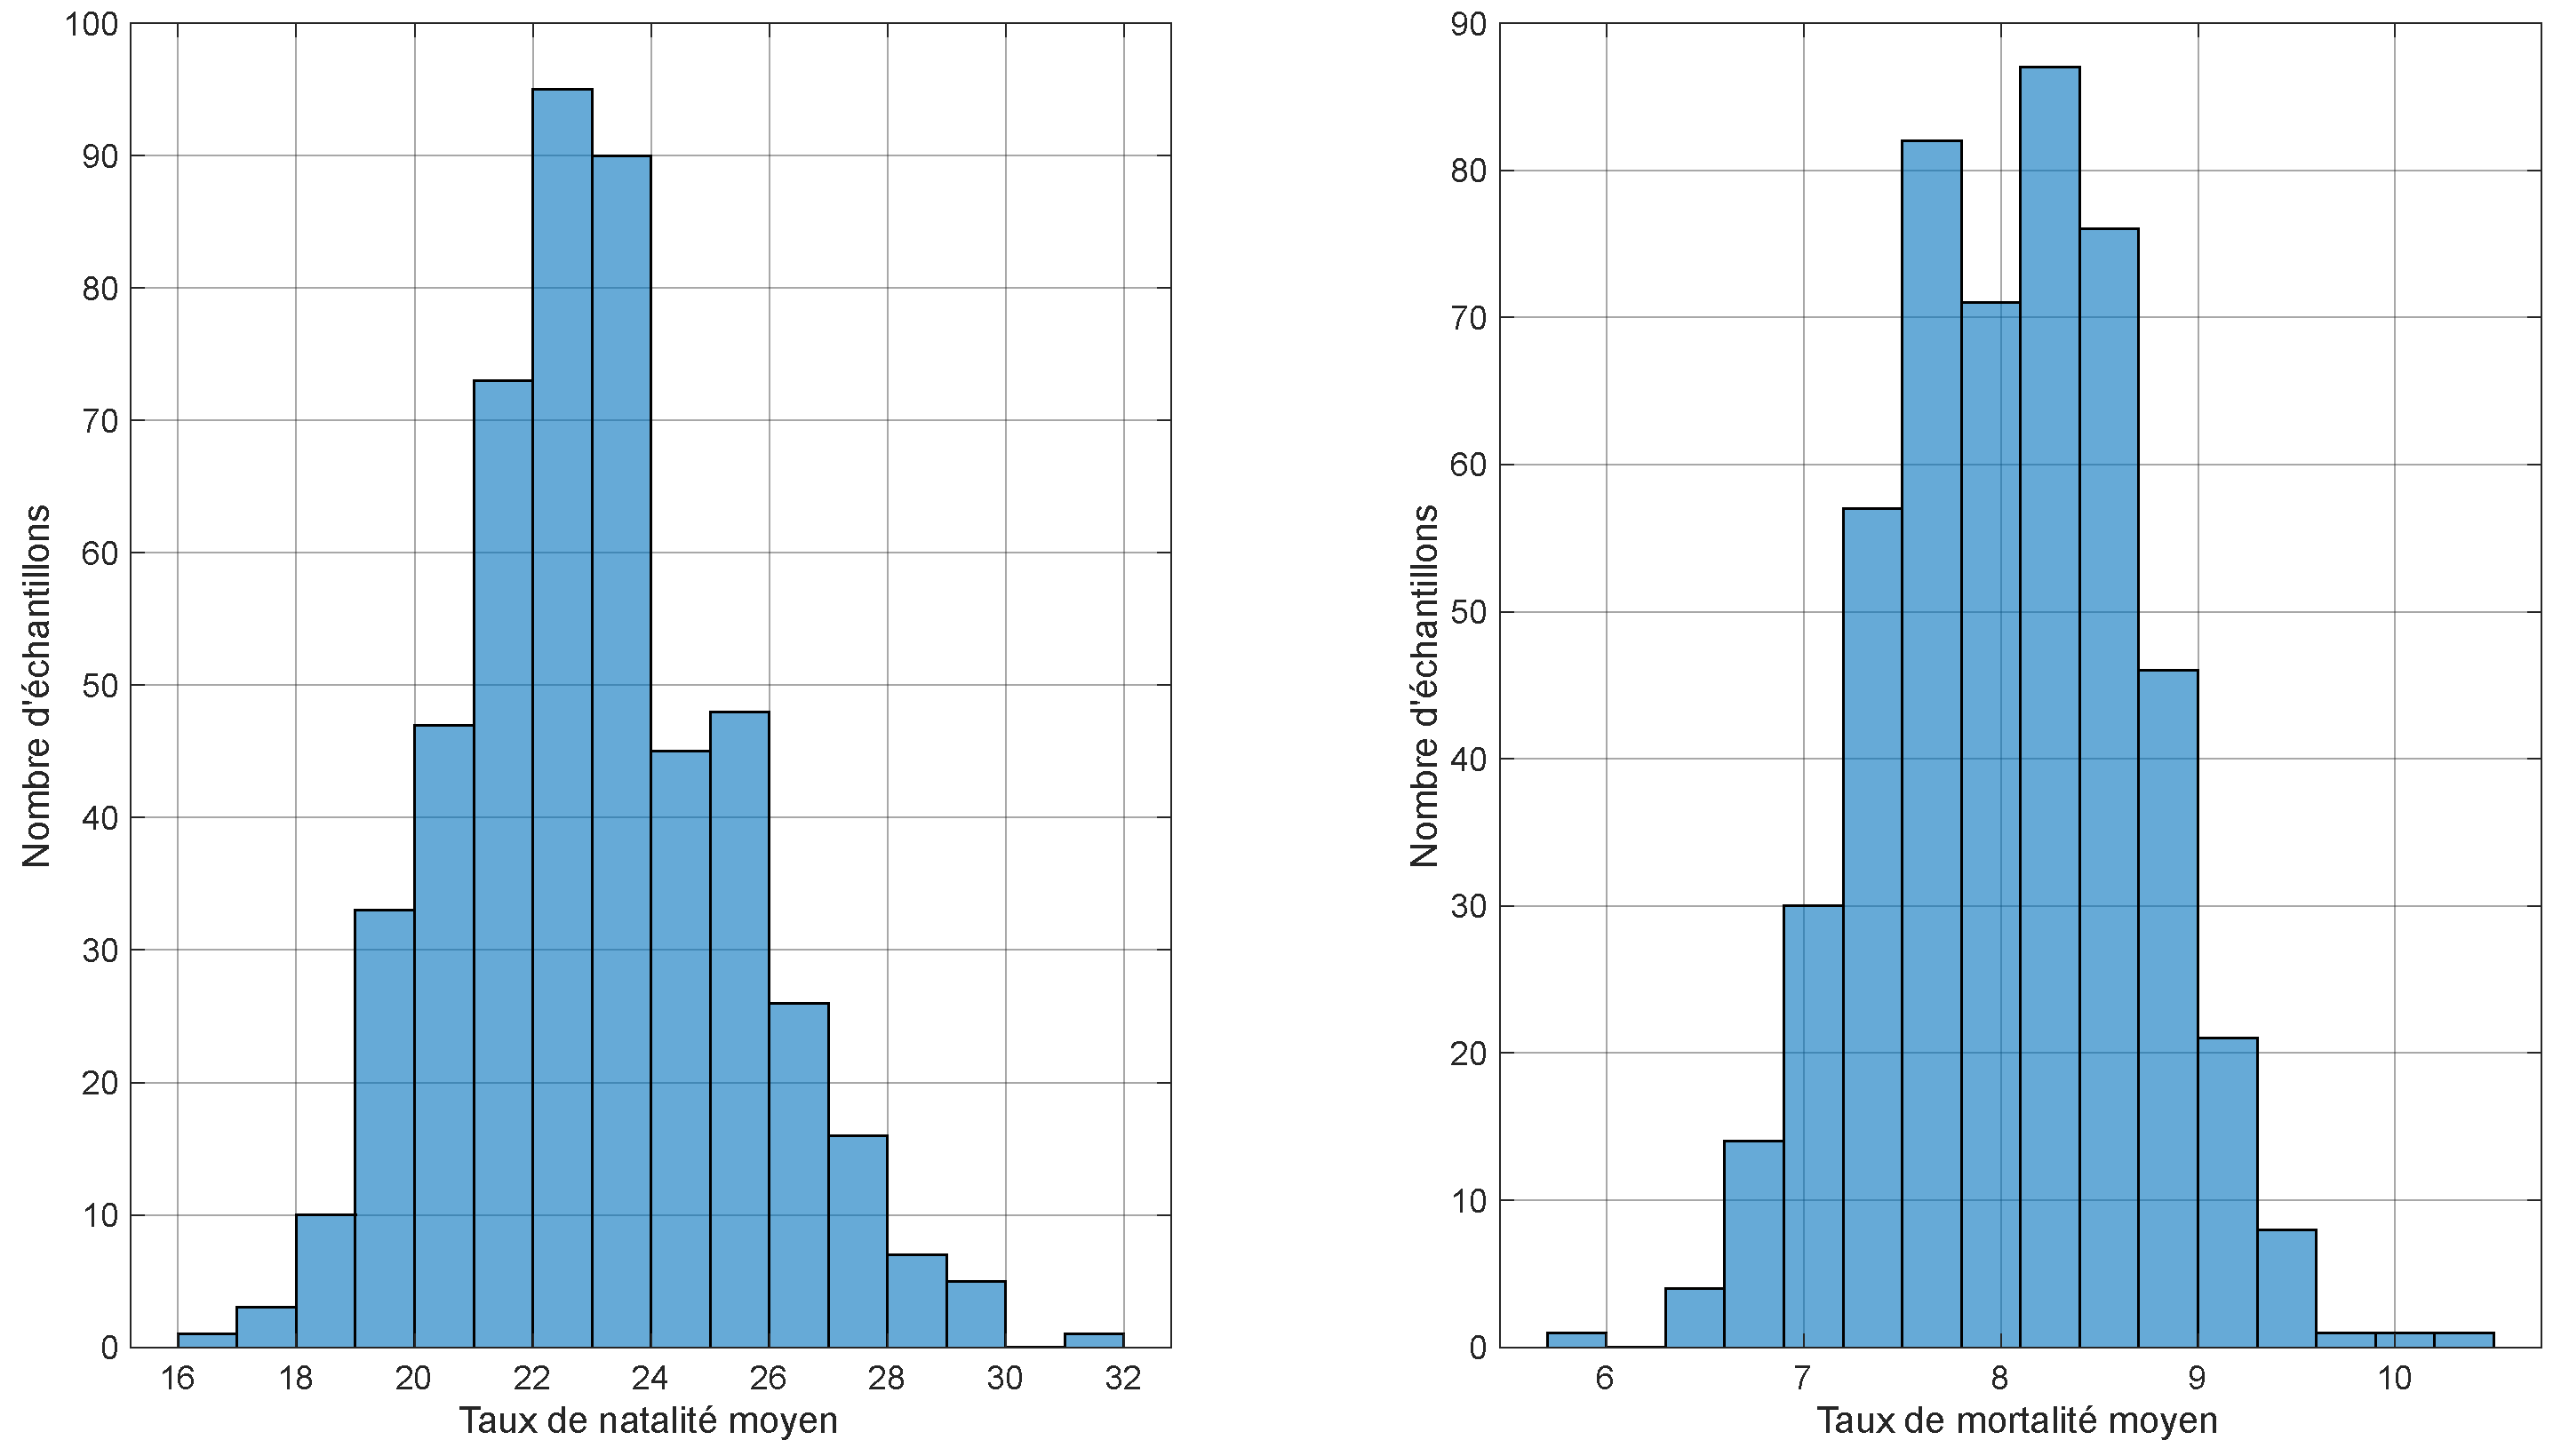
\includegraphics[width=\textwidth]{resources/pdf/figures/Q2bi.pdf}
	    \caption{Histogrammes des taux moyens de 500 échantillons i.i.d.}
	    \label{fig:Q2bi}
	\end{figure}
	
	Les moyennes des nouvelles variables sont données à la table \ref{tab:Q2bi}.\par
	
	\begin{table}[!ht]
	    \centering
	    \begin{tabular}{|c|c|}
	        \hline
	        \textbf{Taux} & \textbf{Valeur moyenne des échantillons} \(\left [\text{\textperthousand} \right ]\)\\ \hline
	        \hline
	        Taux de natalité & \num{23.1286}\\ \hline
	        Taux de mortalité & \num{8.0051}\\ \hline
	    \end{tabular}
	    \caption{Valeurs moyennes des taux moyens de 500 échantillons i.i.d.}
	    \label{tab:Q2bi}
	\end{table}
	
	En comparaison avec les taux moyens de la population, ces deux moyennes de taux moyens des échantillons sont toutes deux extrêmement proches des valeurs de la population. Alors que les taux pour un échantillon étaient acceptables par rapport à ceux de la population, ceux calculés sur \num{500} échantillons sont très précis. Ce résultat est logique puisque l'on travaille sur un nombre de données beaucoup plus grand, donc se rapprochant beaucoup plus de la population.
	
	\subsubsection{Étude de la médiane du taux de natalité et de mortalité}
	Les deux histogrammes des médianes sont visibles à la figure \ref{fig:Q2bii}. De nouveau, on distingue clairement des allures de loi normales. À noter que celle du taux de natalité est fort piquée.
	
	\begin{figure}[!ht]
	    \centering
	    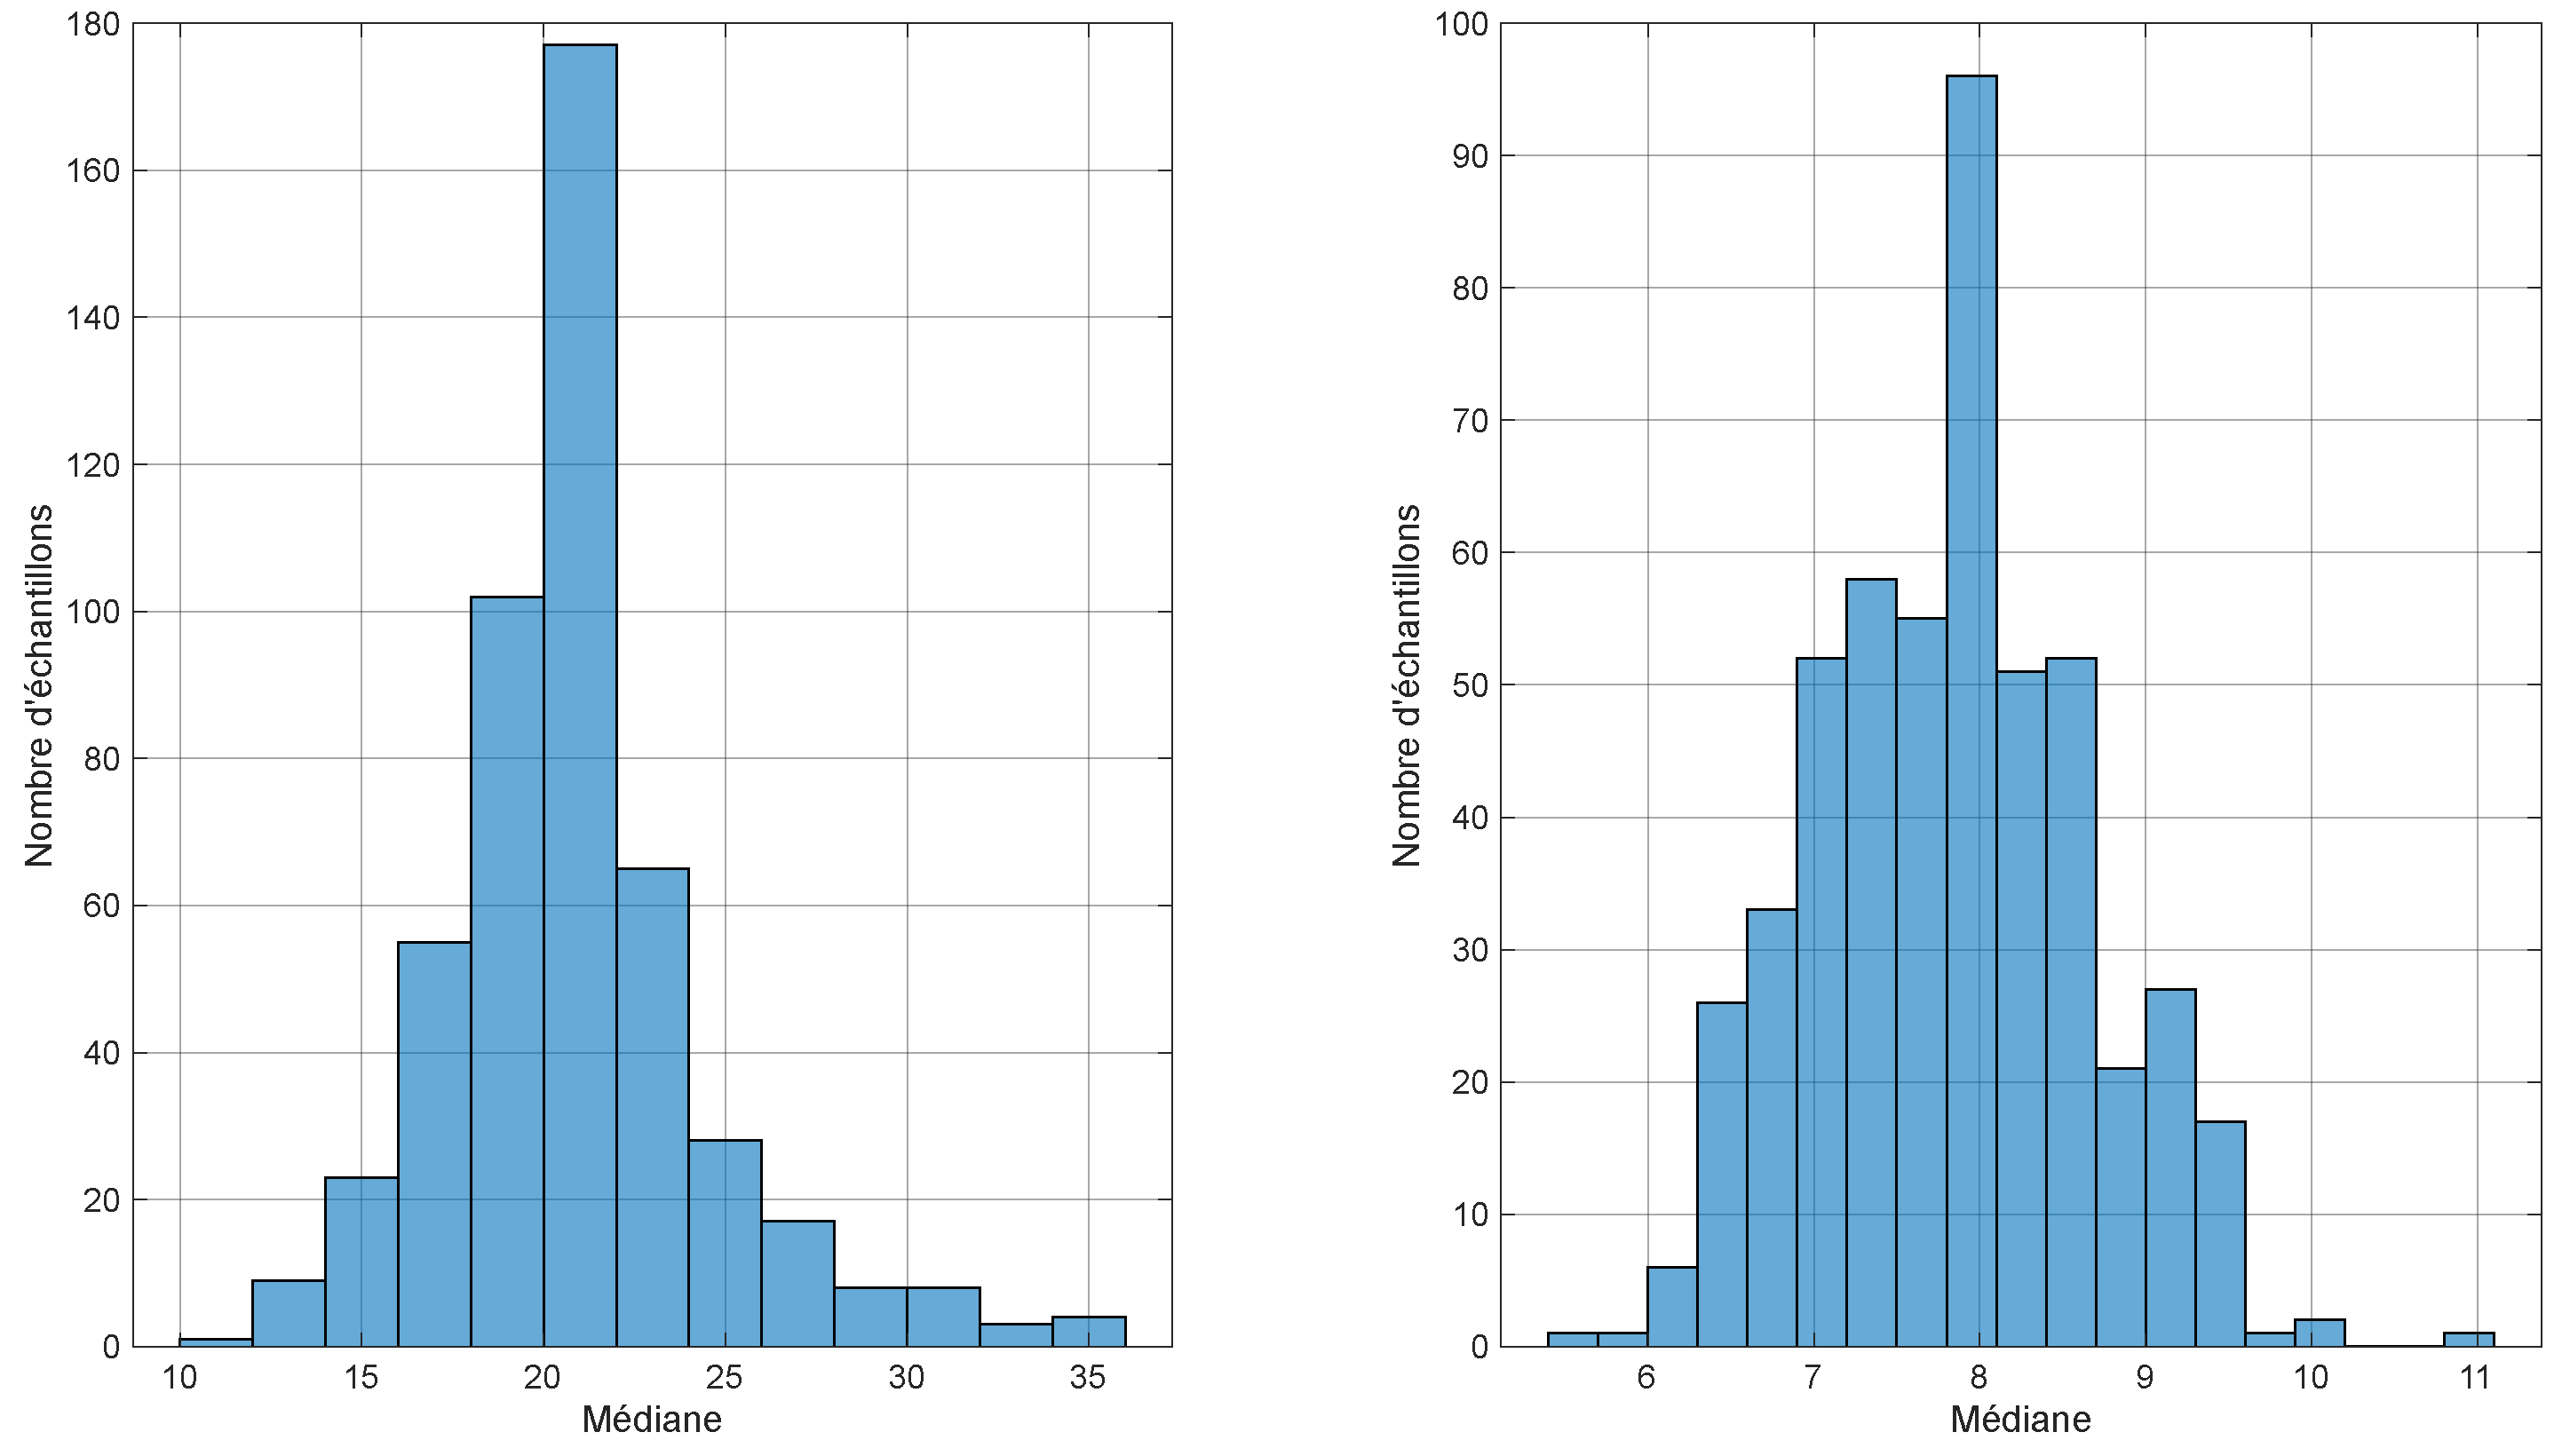
\includegraphics[width=\textwidth]{resources/pdf/figures/Q2bii.pdf}
	    \caption{Histogrammes des médianes de 500 échantillons i.i.d.}
	    \label{fig:Q2bii}
	\end{figure}
	
	Les moyennes des nouvelles variables sont données à la table \ref{tab:Q2bii}.\par
	
	\begin{table}[!ht]
	    \centering
	    \begin{tabular}{|c|c|}
	        \hline
	        \textbf{Taux} & \textbf{Valeur moyenne des échantillons} \(\left [\text{\textperthousand} \right ]\)\\ \hline
	        \hline
	        Taux de natalité & \num{20.8635}\\ \hline
	        Taux de mortalité & \num{7.7869}\\ \hline
	    \end{tabular}
	    \caption{Valeurs moyennes des médianes de 500 échantillons i.i.d.}
	    \label{tab:Q2bii}
	\end{table}
	
	On constate que ces valeurs sont moins proches des moyennes de la population que les valeurs calculées à la section \ref{subsec:Q2bi}. La médiane est donc, dans ce cas, un moins bon estimateur du taux moyen de la population que la moyenne.\par
	
	On note que cela n'est pas toujours le cas, les données aberrantes pouvant influencer les résultats. En effet, la médiane étant peu touchée par les données aberrantes, elle est souvent meilleur estimateur que la moyenne. Cependant, dans la base de données étudiée ici, il n'y a pas de données aberrantes.
	
	\subsubsection{Étude de l'écart-type du taux de natalité et mortalité}
	Les deux graphes sont présentés à la figure \ref{fig:Q2biii}.
	
	Bien que leurs allures fassent penser à une loi normales, ce n'est pas le cas ici. En effet, il a été vu que le carré de \(s_X\) suit une loi \textit{Chi-carré} à \(n-1\) degrés de liberté. Il n'est donc pas possible que \(s_X\) suive une loi normale.\par
	
	\begin{figure}[!ht]
	    \centering
	    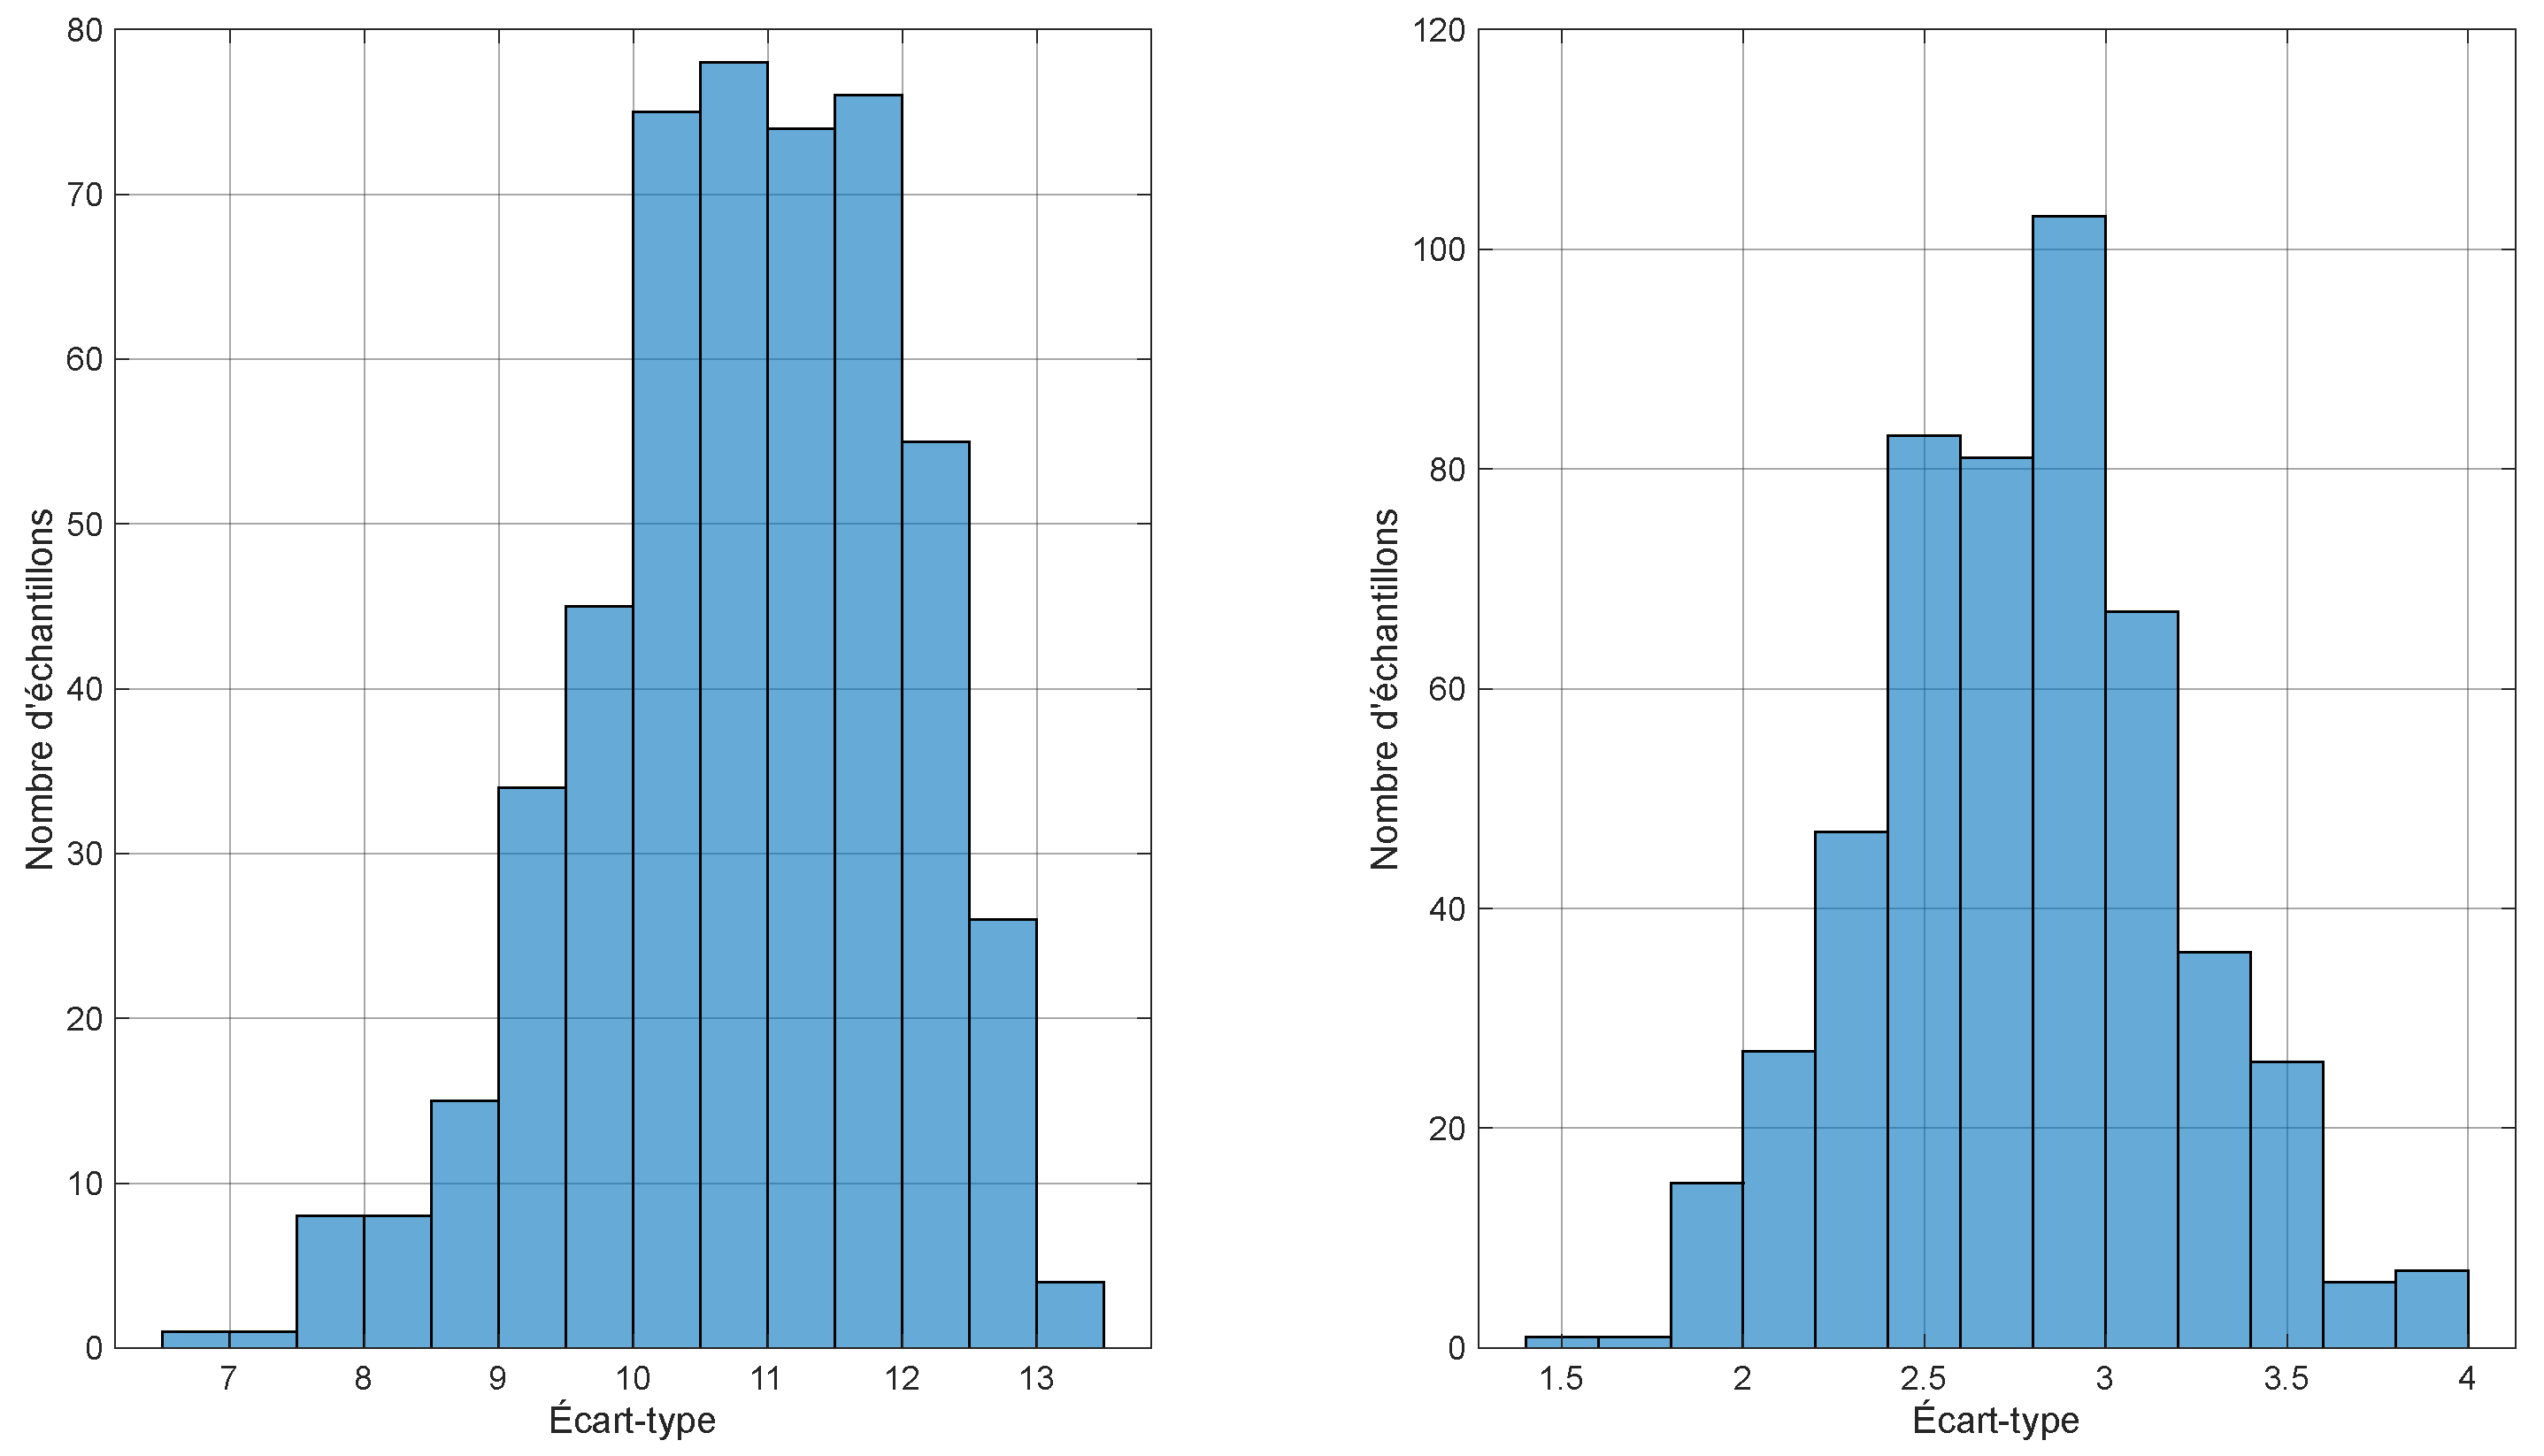
\includegraphics[width=\textwidth]{resources/pdf/figures/Q2biii.pdf}
	    \caption{Histogrammes des écarts-types de \num{500} échantillons i.i.d.}
	    \label{fig:Q2biii}
	\end{figure}
	
	Les moyennes des nouvelles variables sont données à la table \ref{tab:Q2biii}.
	
	\begin{table}[!ht]
	    \centering
	     \begin{tabular}{|c|c|}
	        \hline
	        \textbf{Taux} & \textbf{Valeur moyenne des échantillons} \(\left [\text{\textperthousand} \right ]\)\\ \hline
	        \hline
	        Taux de natalité & \num{10.8078}\\ \hline
	        Taux de mortalité & \num{2.7802}\\ \hline
	    \end{tabular}
	    \caption{Valeurs moyennes des écarts-types de 500 échantillons i.i.d.}
	    \label{tab:Q2biii}
	\end{table}
	
	Les valeurs moyennes des écarts-types des taux de natalité et de mortalité de \num{500} échantillons se rapprochent des écarts-types de la population. On remarque cependant que ces estimations sous-estiment les valeurs de la population. Pour amoindrir cela, on aurait pu utiliser les variances corrigées \(s^2_{n-1}\) des échantillons, qui sont des estimateurs non biaisés de la variance de la population. Cependant, vu l'inégalité de Jensen, l'écart-type \(s_{n-1}\) sous estime également l'écart-type de la population.
	
	\subsubsection{Étude de la distance de Kolmogorv-Smirnov}
	Les graphes présentés à la figure \ref{fig:Q2biv} explicitent les distances de Kolmogorov-Smirnov entre les polygones des fréquences cumulées de la population et des échantillons.\par
	
	L'allure de ces graphes s'apparente à une loi normale, mais légèrement asymétrique par rapport aux valeurs les plus représentées. Concernant le taux de naissance, la distance la plus courante semble valoir environ \num{0.15}, signifiant, qu'en moyenne, il y a \num{0.15} d'écart entre la population et un échantillon aléatoire i.i.d. quelconque de \num{20} pays. Pour le taux de mortalité, cet écart moyen semble être d'environ \num{0.8}.
	
	\begin{figure}[!ht]
	    \centering
	    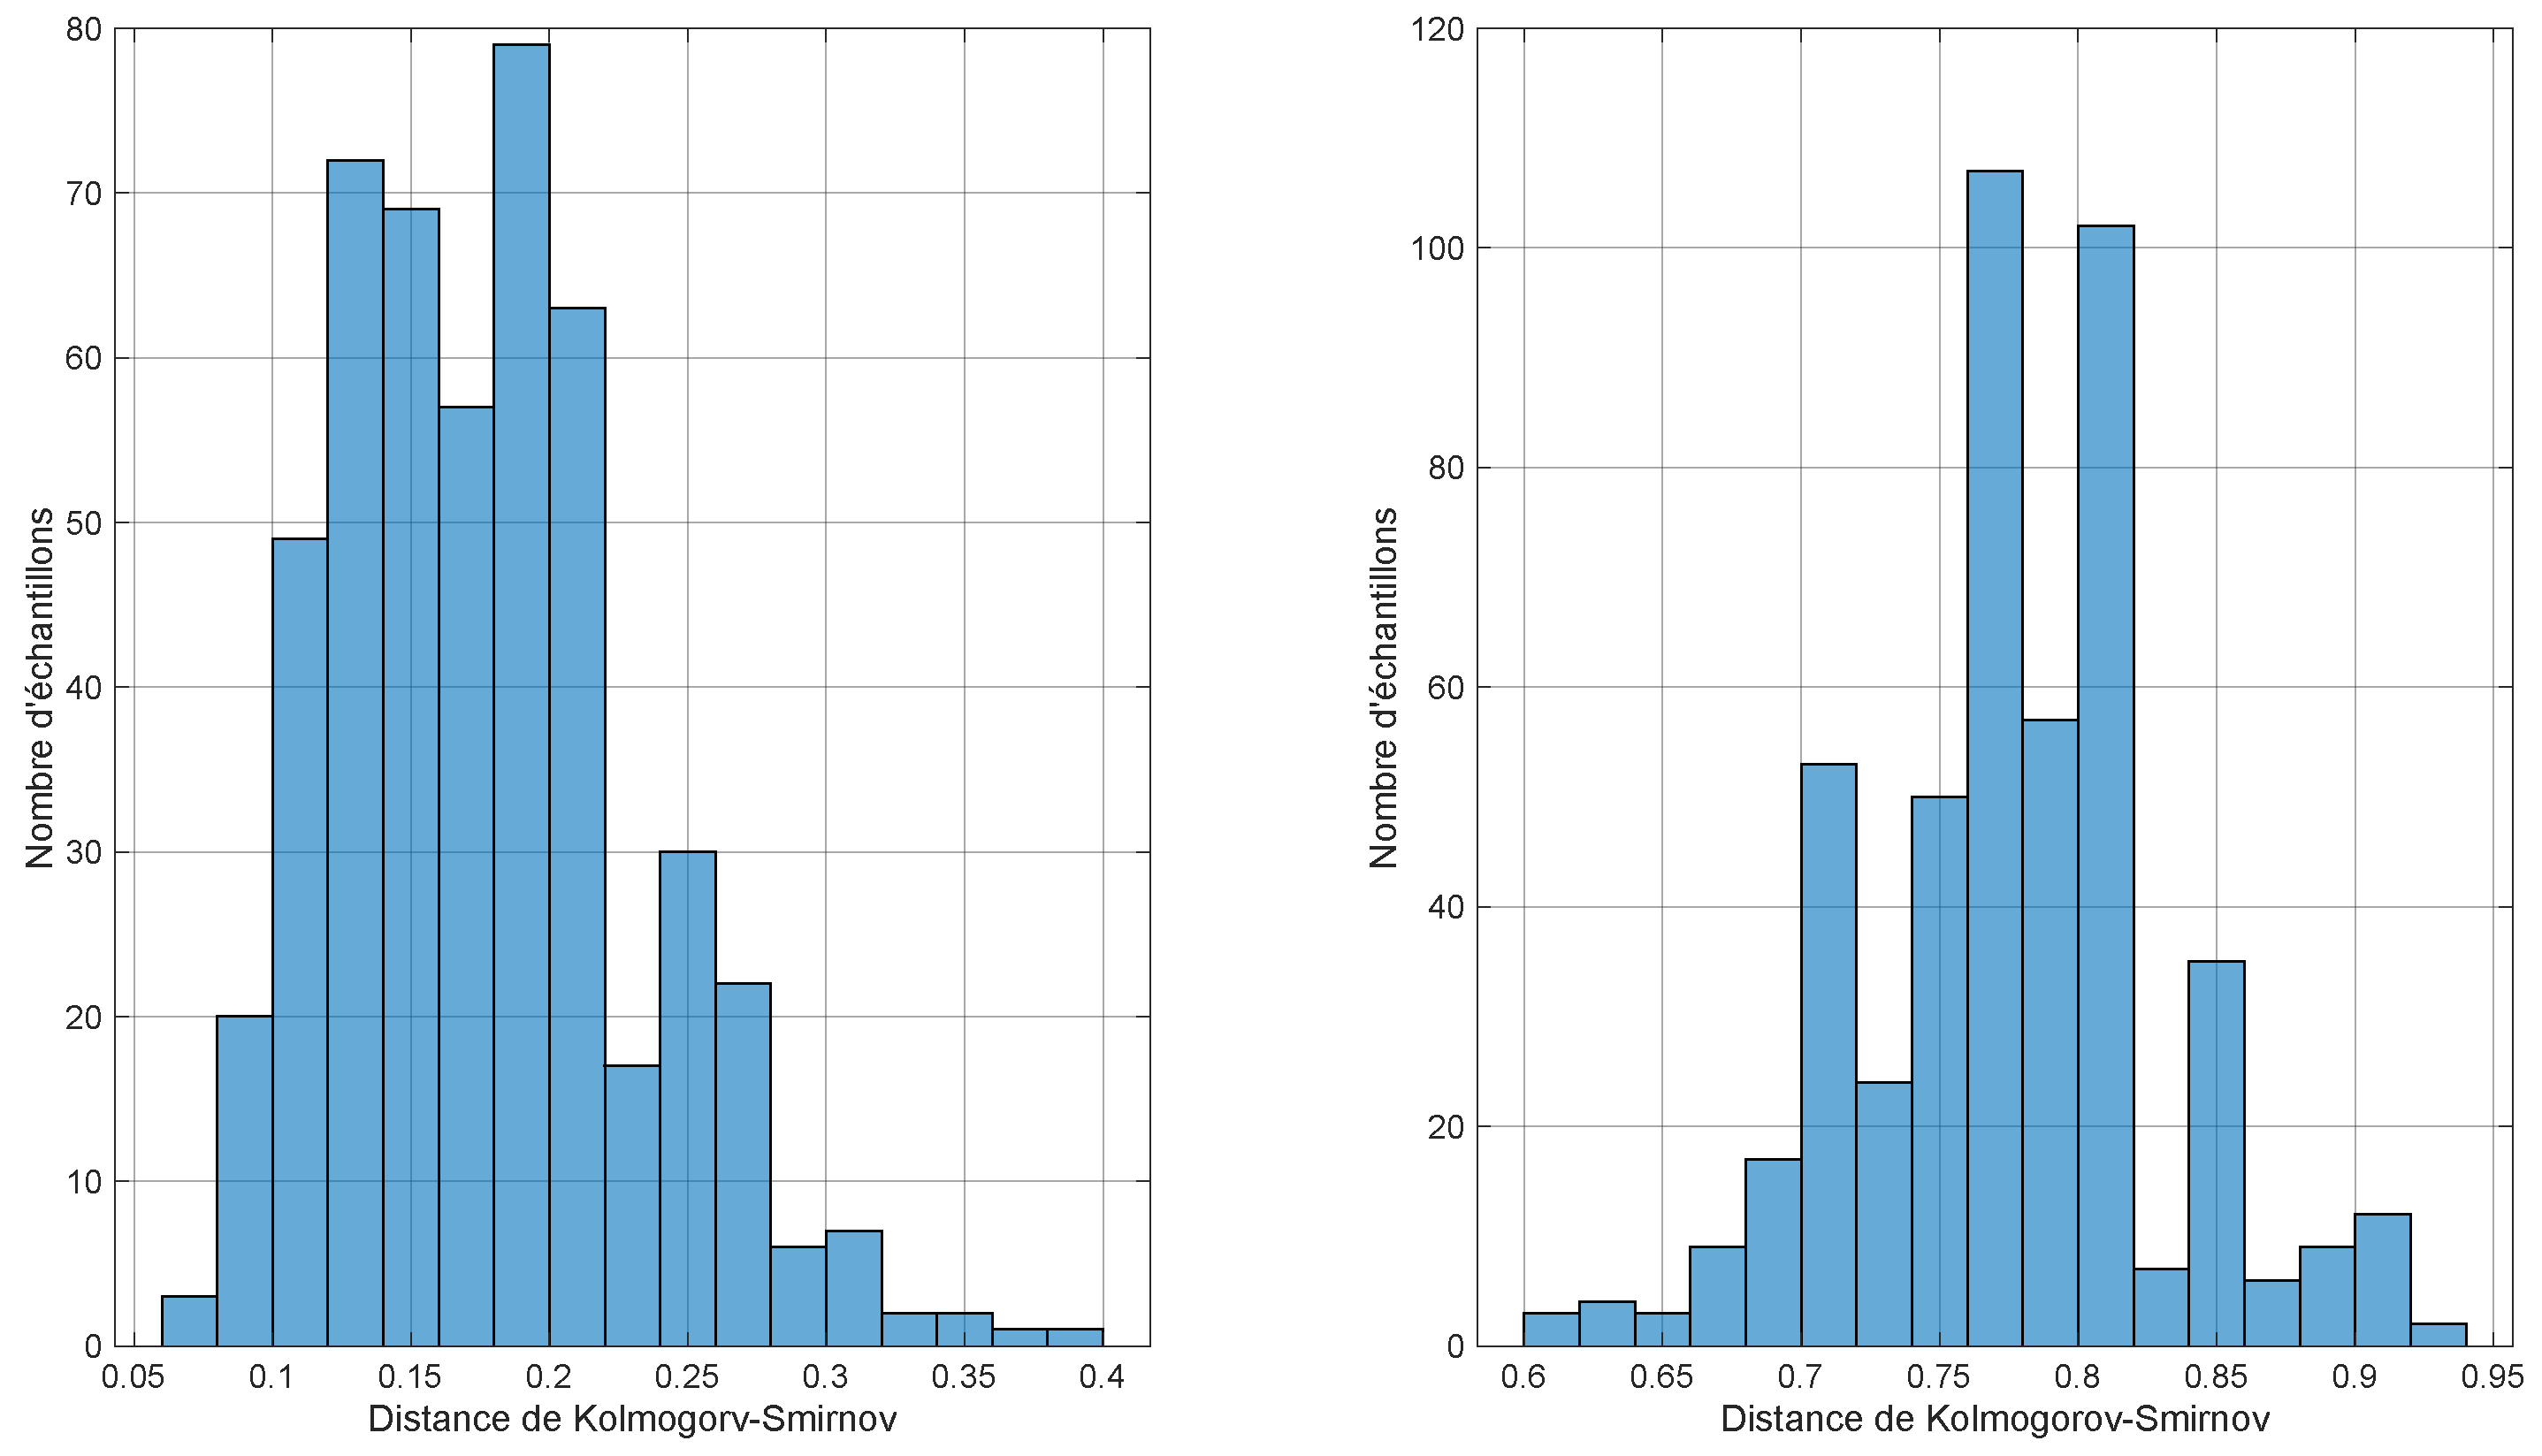
\includegraphics[width=\textwidth]{resources/pdf/figures/Q2biv.pdf}
	    \caption{Histogrammes des distances de Kolmogorov-Smirnov de 500 échantillons i.i.d.}
	    \label{fig:Q2biv}
	\end{figure}
	
	
	% ---------- Estimation ---------- %
	\section{Estimation}
	On tire, grâce à la fonction auxiliaire \hyperref[subsec:code-auxiliary]{\texttt{getsample}}, 100 échantillons i.i.d. de 20 pays. On ne considère, pour les sous-sections suivantes, que le taux de natalité.
	
	% Question 3 - a)
	\subsection{Utilisation de la moyenne comme estimateur}
	\label{subsec:Q3a}
	On choisit la moyenne \(m_X\) des échantillons comme estimateur. Le script \hyperref[subsec:code-Q3]{\texttt{Q3abd}} calcule ces moyennes et les enregistre dans une nouvelle variable. Le biais et la variance de l'estimateur sont calculés par le biais de cette nouvelle variable.\par
	
	L'erreur quadratique d'une estimation est donnée par
	\begin{align}
	    \label{eq:Q3a}
	    E\left\{\left (\T_n-\theta^*\right )^2\right\} &= V\left\{\T_n\right\} + \left (E\left\{\T_n-\theta^*\right\}\right)^2\\
	    \nonumber&= \text{Variance} + \text{Biais}^2
	\end{align}
	avec
	
	\begin{itemize}
	    \item \(\T_n\), l'estimateur;
	    \item \(\theta^*\), la vraie valeur à estimer.
	\end{itemize}
	
	Dans ce cas-ci, l'estimateur est la moyenne \(m_X\) et la vraie valeur à estimer est la moyenne \(\mu\) de la population.\par
	
	On peut alors, en reprenant les expression de l'équation \eqref{eq:Q3a}, calculer le biais et la variance de l'estimateur \(m_X\):
	
	\begin{itemize}
	    \item biais: \(\left |E\left\{m_X-\mu\right\}\right |\);
	    \item variance: \(V\left\{m_X\right\} = E\left \{\left (m_x - E\left \{m_x\right\}\right )^2\right \}\).
	\end{itemize}
	
	La moyenne \(\mu\) de la population étant connue (calculée à la section \ref{subsec:Q1b}), on obtient les résultats présentés à la table \ref{tab:Q3a}.\par
	
	\begin{table}[!ht]
	    \centering
	    \begin{tabular}{|c|c|c|}
	        \hline
	        \textbf{Estimateur} & \textbf{Biais} \(\left [\text{\textperthousand} \right ]\) & \textbf{Variance} \(\left [\text{\textperthousand}^2 \right ]\)\\ \hline
	        \hline
	        Moyenne \(m_X\) & \num{0.1254} & \num{6.4093}\\ \hline
	    \end{tabular}
	    \caption{Biais et variance de l'estimateur \(m_X\) du taux de natalité moyen de la population.}
	    \label{tab:Q3a}
	\end{table}
	
	Comme attendu au vu des résultats de la section \ref{subsec:Q2bi}, on constate que le biais de l'estimateur moyenne est très faible par rapport à la moyenne de la population. La variance, quant à elle, semble tourner autour de la valeur \num{6.5}. L'écart-type, obtenu en prenant la racine carrée de cette valeur, est plutôt petit traduisant un étalement assez faible des valeurs de \(m_X\).\par
	
	L'erreur quadratique peut également être calculée et vaut \num{7.8014}.
	
	% Question 3 - b)
	\subsection{Utilisation de la médiane comme estimateur}
	\label{subsec:Q3b}
	On choisit la médiane \(median_X\) des échantillons comme estimateur. Le script \hyperref[subsec:code-Q3]{\texttt{Q3abd}} calcule ces médianes et les enregistre dans une nouvelle variable. Le biais et la variance de l'estimateur sont calculés par le biais de cette nouvelle variable.\par
	
	En procédant de la même manière qu'à la section \ref{subsec:Q3a}, on trouve:
	
	\begin{itemize}
	    \item biais: \(\left |E\left\{median_X-\mu\right\}\right |\);
	    \item variance: \(V\left\{median_X\right\} = E\left \{\left (median_x - E\left \{median_x\right\}\right )^2\right \}\).
	\end{itemize}
	
	On obtient alors les résultats présentés à la table \ref{tab:Q3b}.\par
	
	\begin{table}[!ht]
	    \centering
	    \begin{tabular}{|c|c|c|}
	        \hline
	        \textbf{Estimateur} & \textbf{Biais} \(\left [\text{\textperthousand} \right ]\) & \textbf{Variance} \(\left [\text{\textperthousand}^2 \right ]\)\\ \hline
	        \hline
	        Médiane \(median_X\) & \num{0.7430} & \num{15.6342}\\ \hline
	    \end{tabular}
	    \caption{Biais et variance de l'estimateur \(median_X\) du taux de natalité moyen de la population.}
	    \label{tab:Q3b}
	\end{table}
	
	On constate que le biais et la variance de \(median_X\) sont plus élevés que ceux de \(m_X\). L'étalement des valeurs de \(median_X\) est plus important.\par
	
	L'erreur quadratique vaut, quant à elle, \num{15.1499}. À première vue, on observe que \(median_X\) est un moins bon estimateur que \(m_X\).
	
	% Question 3 - c)
	\subsection{Estimateurs sur des échantillons i.i.d. de taille \num{50}}
	En procédant de la même manière qu'aux sections \ref{subsec:Q3a} et \ref{subsec:Q3b} avec des échantillons i.i.d. de 50 pays, on obtient, via le script \hyperref[subsec:code-Q3]{\texttt{Q3c}}, les résultats présentés à la table \ref{tab:Q3c}.\par
	
	\begin{table}[!ht]
	    \centering
	    \begin{tabular}{|c|c|c|}
	        \hline
	        \textbf{Estimateur} & \textbf{Biais} \(\left [\text{\textperthousand} \right ]\) & \textbf{Variance} \(\left [\text{\textperthousand}^2 \right ]\)\\ \hline
	        \hline
	        Moyenne \(m_X\) & \num{0.0796} & \num{2.2881}\\ \hline
	        Médiane \(median_X\) & \num{0.1740} & \num{3.0515}\\ \hline
	    \end{tabular}
	    \caption{Biais et variance des estimateurs \(m_X\) et \(median_X\) du taux de natalité moyen de la population pour des échantillons i.i.d. de 50 pays.}
	    \label{tab:Q3c}
	\end{table}
	
	On constate tout d'abord que le biais et la variance de l'estimateur \(m_X\) sont plus petits que ceux de \(median_X\), confirmant l'observation de la section \ref{subsec:Q3b} comme quoi \(m_X\) est un meilleur estimateur que \(median_X\).\par
	
	On constate également que les \num{4} valeurs obtenues sont plus petites que celles calculées aux sections \ref{subsec:Q3a} et \ref{subsec:Q3b}, traduisant des résultats d'une précision plus importante. Cette diminution des valeurs est la conséquence logique de l'augmentation de la taille des échantillons.\par
	
	Plus la taille de l'échantillon augmente, plus le biais de l'estimateur \(m_X\) diminue et tend en fait vers \(0\). La moyenne de cet estimateur tend donc vers la moyenne de la population.\par
	
	Enfin, on remarque que, pour chacun des estimateurs, la variance diminue lorsque la taille de l'échantillon augmente. En effet, il parait logique que les valeurs des moyennes et médianes soient moins dispersées lorsque l'on considère de plus grands échantillons.
	
	% Question 3 - d)
	\subsection{Construction d'intervalles de confiance}
	Dans cette partie, on travaille de nouveau avec 100 échantillons i.i.d. de 20 pays. Les données des sous-sections suivantes ont été obtenues grâce au script \hyperref[subsec:code-Q3]{\texttt{Q3abd}}.\par
	
	Les intervalles de confiance, centré sur \(m_X\), étant à \num{95}\% du taux de natalité de la population, on peut d'ors et déjà définir que le paramètre \(\alpha\) vaut \(\num{1} - \num{0.95} = \num{0.05}\).
	
	\subsubsection{Loi de Student}
	L'intervalle de confiance construit avec la loi de Student est donné par
	\begin{displaymath}
	    \left [m_X-t_{1-\frac{\alpha}{2}}\frac{s_{n-1}}{\sqrt{n}}; m_X+t_{1-\frac{\alpha}{2}}\frac{s_{n-1}}{\sqrt{n}}\right ]
	\end{displaymath}
	En prenant un degré de liberté égale à la taille des échantillons - \num{1}, à savoir \num{19}, dans le cas demandé, on a
	
	\begin{itemize}
	    \item \(n = \num{20}\), la taille des échantillons;
	    \item \(m_X\), la moyenne des échantillons;
	    \item \(t_{1-\frac{\alpha}{2}} = t_{\num{0.975}} = \num{2.093}\), calculé avec la fonction \texttt{tinv}. Cette valeur pourrait également être lue dans une table de données;
	    \item \(s_{n-1}\), l'écart-type corrigé des échantillons, calculée avec la fonction \texttt{std}.
	\end{itemize}
	
	On peut dès lors construire un intervalle de confiance pour chaque échantillon. On constate, en effectuant plusieurs tests, que le nombre d'intervalles de confiance contenant la valeur de la population varie entre \num{88} et \num{98}.
	
	\subsubsection{Loi de Gauss}
	L'intervalle de confiance construit avec la loi de Gauss est donné par
	\begin{displaymath}
	    \left [m_X-u_{1-\frac{\alpha}{2}}\frac{\sigma}{\sqrt{n}}; m_X+u_{1-\frac{\alpha}{2}}\frac{\sigma}{\sqrt{n}}\right ]
	\end{displaymath}
	Dans le cas demandé, on a
	
	\begin{itemize}
	    \item \(n = \num{20}\), la taille des échantillons;
	    \item \(m_X\), la moyenne des échantillons;
	    \item \(u_{1-\frac{\alpha}{2}} = u_{\num{0.975}} = \num{1.96}\), calculé avec la fonction \texttt{normiv}. Cette valeur pourrait également être lue dans une table de données;
	    \item \(\sigma\), l'écart-type de la population, calculée à la section \ref{subsec:Q1b}.
	\end{itemize}
	
	On peut dès lors construire un intervalle de confiance pour chaque échantillon. On constate, dans ce cas, que le nombre d'intervalles de confiance contenant la valeur de la population varie entre \num{93} et \num{99}.\par
	
	Bien que le nombre d'intervalles contenant la valeur de la population varie dans les deux cas, il semblerait que les intervalles construits avec la loi de Gauss sont, de manière générale, plus proche des \num{95}\% attendus.\par
	
	Une loi de Student utilise moins d'informations qu'une loi de Gauss et est donc par conséquent plus générale et moins précise. Au vu des résultats des intervalles construits avec la loi de Gauss, il semblerait qu'il était raisonnable de supposer que la variable parente était Gaussienne.
	
	
	% ---------- Tests d'hypothèse - proportion ---------- %
	\section{Tests d'hypothèse - proportion}
	On tire, grâce à la fonction auxiliaire \hyperref[subsec:code-auxiliary]{\texttt{getsample}}, 100 fois 5 échantillons i.i.d. de 40 pays. Le premier échantillon de chaque tirage est celui de la Belgique; les autres sont ceux des instituts. Tous les résultats des sous-sections suivantes ont été obtenus par le biais du script \hyperref[subsec:code-Q4]{\texttt{Q4ab}}.\par
	
	Au vu des hypothèses à tester, il s'agit de réaliser un test d'hypothèses unilatéral à droite sur une proportion. L'hypothèse \(H_0\) est la suivante: \og la proportion de pays ayant un taux de natalité plus faible que la Belgique est de \(x\)\%\fg{}.\par
	
	Premièrement, on calcule cette valeur \(x\), à savoir la vraie proportion de pays, dans la population, ayant un taux de natalité plus faible que la Belgique. On trouve \(x=\num{21}\%\).\par
	
	Deuxièmement, on calcule la borne supérieure de l'intervalle favorable à \(H_0\), avec un seuil de signification de \(\alpha = \num{5}\%\) et une taille d'échantillon \(n = \num{40}\):
	\begin{align*}
	    x + u_{\num{0.975}}\sqrt{\frac{x\left (\num{1}-x\right )}{n}} &= \num{0.21} + \num{1.96}\sqrt{\frac{\num{0.21}\left (\num{1}-\num{0.21}\right)}{\num{40}}}\\
	    &= \num{0.3362}
	\end{align*}
	Troisièmement, pour chaque échantillon de chaque tirage, on calcule la proportion \(p\) de pays ayant un taux de natalité inférieur à celui de la Belgique. L'hypothèse \(H_0\) sera rejetée si la proportion \(p\) est supérieure à la valeur de la borne supérieure, c'est-à-dire si \(p > 0.3362\).\par
	
	Si on définit une variable aléatoire \(\X\) qui vaut \num{1} si un pays tiré au hasard possède un taux de natalité inférieur à celui de la Belgique et qui vaut \num{0} dans les autres cas, cette variable \(\X\) sera une variable binomiale. De ce fait, si l'hypothèse \(H_0\) est vérifiée, la moyenne et l'écart-type de \(\X\) seront donnés par:
	
	\begin{itemize}
	    \item moyenne: \(x\);
	    \item écart-type: \(\sqrt{x\left (1-x\right)}\).
	\end{itemize}
	
	Lors de la construction de la borne supérieur de l'intervalle, on a approximé une loi binomiale par une loi normale. Cela n'est valable que si \(\text{min}\left (nx; n\left (1-x\right )\right)\geq 5\), ce qui est bien le cas.
	
	% Question 4 - a)
	\subsection{Rejet de l'hypothèse par l'État belge}
	\label{subsec:Q4a}
	De multiples tests montrent que l'État belge rejette l'hypothèse entre \num{0} et \num{7} fois sur \num{100}. En moyenne, le pourcentage de rejet est proche du seuil \(\alpha\) fixé mais lui reste néanmoins pratiquement toujours inférieur. Cette différence par rapport à \(\alpha\) peut être due à l'approximation de la loi binomiale par une loi normale.
	
	% Question 4 - b)
	\subsection{Rejet de l'hypothèse par l'O.M.S.}
	Afin de connaître le nombre de rejet de l'hypothèse \(H_0\) par l'O.M.S., on comptabilise le nombre de tirages où au moins un des quatres instituts a rejeté l'hypothèse \(H_0\).\par
	
	De multiples tests montrent que le nombre de fois où l'O.M.S. a considéré que les belges n'ont pas un faible taux de natalité varie entre \num{5} et \num{17} fois sur \num{100}.\par
	
	On constate premièrement que cette proportion est, en moyenne, supérieure à \(\alpha\). Ce résultat parait logique puisque les 4 instituts possèdent chacun un échantillon différent et qu'il suffit qu'un seul des 4 rejette l'hypothèse. La probabilité que cela arrive est supérieure à la probabilité que l'État belge rejette l'hypothèse.\par
	
	En effet, la probabilité qu'un échantillon rejette l'hypothèse étant de \(\alpha = \num{0.05}\), on calcule
	\begin{equation}
	    \label{eq:Q4b}
	    1 - \left (1-0.05\right )^4 = \num{0.1855} > \alpha
	\end{equation}
	On constate néanmoins que la probabilité \eqref{eq:Q4b} calculée ne correspond pas tout à fait au nombre de fois où l'O.M.S. a considéré que l'État belge avait un faible taux de naissance. Cela reflette, une fois de plus, l'imprécision des résultats due à l'approximation de la loi binomiale par une loi normale.
	
	% Question 4 - c)
	\subsection{Méthodes alternatives}
	Pour éviter que les instituts de statistique indépendants soient avantagés par rapport à l'État belge, plusieurs méthodes auraient pu être utilisées:
	
	\begin{itemize}
	    \item on aurait pu imposer à chaque institut de travailler sur le même échantillon;
	    \item on aurait pu, tout en gardant le seuil de signification \(\alpha\) pour l'État belge, diminuer le seuil de signification des autres instituts, réduisant ainsi la taille de leur intervalle favorable à \(H_0\). On pourrait, par exemple, choisir un seuil tel que la probabilité \eqref{eq:Q4b} soit égale à la probabilité que l'État belge rejette l'hypothèse \(H_0\);
	    \item à l'inverse, on aurait pu augmenter le seuil de signification de l'État belge tout en gardant le seuil \(\alpha\) pour les autres instituts;
	    \item on aurait pu également augmenter le nombre de données sur lesquelles a travaillé l'État belge, c'est-à-dire soit augmenter la taille de l'échantillon, soit travailler sur plusieurs échantillons. En effet, plus elle aura accès à un grand nombre de données, plus les résultats trouvés seront proches de la réalité et donc fiables, réduisant ainsi les inégalités avec les autres instituts.
	\end{itemize}
	
	À noter que les solutions augmentant un seuil de signification réduisent la fiabilité des résultats.
	
	
	% ---------- Annexe ---------- %
	\appendix
	\restoregeometry
	
	
	% ---------- Code Matlab ---------- %
	\section*{Code Matlab}
	Les codes Matlab se trouvant dans des dossiers différents, il est impératif de lancer le script \hyperref[subsec:code-auxiliary]{\texttt{startup}}\footnote{Théoriquement, Matlab exécute ce script automatiquement à l'ouverture du projet, mais cela ne pourrait pas être le cas.} en premier.
	
	\subsection*{Scripts}
	
	\subsubsection*{Question 1}
	\label{subsec:code-Q1}
	\lstinputlisting[style=MyMatlab, caption=Script \texttt{Q1a}.]{resources/m/Q1/Q1a.m}
	\lstinputlisting[style=MyMatlab, caption=Script \texttt{Q1b}.]{resources/m/Q1/Q1b.m}
	\lstinputlisting[style=MyMatlab, caption=Script \texttt{Q1c}.]{resources/m/Q1/Q1c.m}
	\lstinputlisting[style=MyMatlab, caption=Script \texttt{Q1d}.]{resources/m/Q1/Q1d.m}
	\lstinputlisting[style=MyMatlab, caption=Script \texttt{Q1e}.]{resources/m/Q1/Q1e.m}
	\lstinputlisting[style=MyMatlab, caption=Script \texttt{Q1f}.]{resources/m/Q1/Q1f.m}
	
	\subsubsection*{Question 2}
	\label{subsec:code-Q2}
	\lstinputlisting[style=MyMatlab, caption=Script \texttt{Q2a}.]{resources/m/Q2/Q2a.m}
	\lstinputlisting[style=MyMatlab, caption=Script \texttt{Q2b}.]{resources/m/Q2/Q2b.m}
	
	\subsubsection*{Question 3}
	\label{subsec:code-Q3}
	\lstinputlisting[style=MyMatlab, caption=Script \texttt{Q3abd}.]{resources/m/Q3/Q3abd.m}
	\lstinputlisting[style=MyMatlab, caption=Script \texttt{Q3c}.]{resources/m/Q3/Q3c.m}
	
	\subsubsection*{Question 4}
	\label{subsec:code-Q4}
	\lstinputlisting[style=MyMatlab, caption=Script \texttt{Q4ab}.]{resources/m/Q4/Q4ab.m}
	
	\subsection*{Scripts et fonctions auxiliaires}
	\label{subsec:code-auxiliary}
	\lstinputlisting[style=MyMatlab, caption=Fonction \texttt{getsample}.]{resources/m/additional/getsample.m}
	\lstinputlisting[style=MyMatlab, caption=Script \texttt{loaddata}.]{resources/m/additional/loaddata.m}
	\lstinputlisting[style=MyMatlab, caption=Script \texttt{startup}.]{resources/m/startup.m}
\end{document}
